
\documentclass[11pt,titlepage,a4paper]{report}

%INCLUSIONE PACCHETTI
%---------------------------------------------
\usepackage[italian]{babel}
\usepackage{fancyhdr}
\usepackage{graphicx}
\graphicspath{{./pics/}} % cartella di salvataggio immagini

% STILE DI PAGINA
%---------------------------------------------
\pagestyle{fancy}
\renewcommand{\sectionmark}[1]{\markright{\thesection.\ #1}}
\lhead{\nouppercase{\rightmark}}
\rhead{\nouppercase{\leftmark}}
\renewcommand{\chaptermark}[1]{%
\markboth{\thechapter.\ #1}{}}

%Ridefinisco lo stile plain della pagina
\fancypagestyle{plain}{%
	\lhead{
\includegraphics[height=50pt]{logo.eps}}
	\chead{}
	\rhead{HappyCode inc \\ happycodeinc@gmail.com}
	\lfoot{BR-jsys}
	\cfoot{\thepage}
	\renewcommand{\headrulewidth}{1pt}
	\renewcommand{\footrulewidth}{1pt}
}
% layout
\begin{document}
%definizione variabili 
\newcommand{\lv}{ 1.5 } % latest version
\newcommand{\dt}{ Specifica Tecnica }% Document title
%common variables
\newcommand{\br}{\underline{business rule}}
\newcommand{\brs}{\underline{business rules}}
\newcommand{\bo}{\underline{business object}}
\newcommand{\bos}{\underline{business objects}}
\newcommand{\rp}{\underline{repository}}
\newcommand{\brp}{BusinessRuleParser}
\newcommand{\brl}{BusinessRuleLexer}
\newcommand{\BR}{\underline{BusinessRule}}

%nomi dei componenti
\newcommand{\AT}{Alessia Trivellato}
\newcommand{\ET}{Elena Trivellato}
\newcommand{\FC}{Filippo Carraro}
\newcommand{\LA}{Luca Appon}
\newcommand{\MB}{Michele Bortolato}
\newcommand{\MT}{Marco Tessarotto}
\newcommand{\MM}{Mattia Meroi}%altre variabili
% ultime versioni dei documenti da modificare solo alla fine
\newcommand{\AR}{AnalisiDeiRequisiti.2.6.pdf}
\newcommand{\DdP}{DefinizioneDiProdotto.0.9.pdf}
\newcommand{\G}{ Glossario.1.8.pdf }
\newcommand{\NdP}{NormeDiProgetto.2.0.pdf}
\newcommand{\PdQ}{ PianoDiQualifica.2.0.pdf }
\newcommand{\PdP}{ PianoDiProgetto.1.7.pdf }
\newcommand{\ST}{SpecificaTecnica.1.5.pdf}
\newcommand{\TR}{TestReport.0.7.pdf}
\newcommand{\MU}{ManualeUtente.0.3.pdf}%nomi documenti
%fine definizione variabili
\hyphenation{
 a-na-lo-go
 as-so-cia-zio-ne
 %attività non si può inserire come tutte le parole accentate che vanno messe nel testo semplice scritte at\-ti\-vi\-tà o come variabile
 coe-ren-za
 com-po-nen-ti
 des-crit-te
 des-cri-zio-ni
 di-a-gram-ma
 di-a-gram-mi
 e-le-men-to
 e-se-gui-re
 e-si-sten-ti
 es-pli-ci-to
 glo-bal-men-te
 glos-sa-rio
 li-vel-lo
 ne-ces-sa-rio
 per-met-te-re
 re-po-si-to-ry
 re-vi-sio-na-men-to
 ri-chies-te
 se-gna-la-ta
 va-li-da-zio-ne
 va-ria-bi-li
 ve-ri-fi-ca-re
 vi-sua-liz-za-te
 e-ven-tua-li
 o-pe-ra-zio-ne
 ar-chi-via-zio-ne
 mo-di-fi-ca
}


%sillabazione
\begin{titlepage}
\begin{center}
\vspace*{0.5in}

\includegraphics{logo.eps}
\vspace*{0.2in}

{\Large \textbf{BR-jsys}}
{\Large \emph{business rules} per sistemi gestionali in architettura J2EE } 
\vspace{2in}

\Huge \textsc{ \dt }

\end{center}
\end{titlepage}
\vspace*{0.5in}%pagina del titolo


\begin{center}
\thispagestyle{plain}
\begin{table}[htbp]
\large{
\begin{tabular}{l}
\Large{\textbf{\textsf{Capitolato: ''BR-jsys``}}} \\
\begin{tabular}{|p{6cm}|p{6cm}|} \hline
\textbf{Data creazione:} & 18/11/2007 \\ \hline
\textbf{Versione:} & \lv \\ \hline
\textbf{Stato del documento:} & formale, esterno \\ \hline
% ----------------------------------------------------------------------------autori
\textbf{Revisione RPD} &   \\ \hline
\textbf{Redazione:} & \MB \\ \hline
\textbf{Revisione:} & \AT , \ET  \\ \hline
\textbf{Approvazione:}  & \MM \\ \hline
\textbf{Revisione RQ} &   \\ \hline
\textbf{Redazione:} & \ET \\ \hline
\textbf{Revisione:} & \FC \\ \hline
\textbf{Approvazione:}  & \AT \\ \hline
\end{tabular} \\
\end{tabular}
}
\end{table}
\end{center}

\begin{center}
\begin{table}[hbtp]
\large{
\begin{tabular}{l}
\large{\textbf{\textsf{Lista di distribuzione}}} \\
\begin{tabular}{|p{6cm}|p{6cm}|} \hline
%  -------------------------------------------------------------lista di distribuzione
{HappyCode inc}& Gruppo di lavoro\\ \hline
{Tullio Vardanega, Renato Conte}& Committente \\ \hline 
{Zucchetti S.r.l}& Azienda proponente\\ \hline
\end{tabular} \\
\end{tabular}
}
\end{table}
\end{center}

\begin{center}
\begin{table}[hbtp]

\Large{\textbf{\textsf{Diario delle modifiche}}} \\
\begin{small}
\begin{tabular}[t]{|p{1,2cm}|p{1.9cm}|p{2.9cm}|p{5cm}|} \hline
Versione & Data & Autore & Descrizione \\ \hline
%-------------------------------------------------------------------------------diario modifiche
1.5 & 07/03/2008 & \ET & Correzione documento\\ \hline
1.4 & 06/03/2008 & \LA & Aggiunto Sommario\\ \hline
1.3 & 06/03/2008 & \MB & Aggiunta diagrammi di stato .\\ \hline
1.2 & 05/03/2008 & \MM & Evidenziazione dei termini contenuti nel documento \G .\\ \hline
1.1 & 04/03/2008 & \MM & Aggiunta di link ipertestuali all'indice del documento.\\ \hline
1.0 & 16/02/2008 & \MB & Inserimento diagramma di collaborazione e diagramma di sequenza. \\ \hline
0.9 & 15/02/2008 & \ET & Correzione grammaticale \\ \hline
0.8 & 12/02/2008 & \MT & Modifiche ai diagrammi di attivit\`a e alle loro descrizioni\\ \hline
0.7 & 08/02/2008 & \MT & Aggiunta dei diagrammi di attivit\`a e rispettive descrizioni\\ \hline
0.6 & 06/02/2008 & \MB & Aggiunta dei diagrammi delle componenti e loro descrizione\\ \hline
0.5 & 05/02/2008 & \MT & Aggiunta del nome del file nel modello di documento\\ \hline
0.4 & 22/01/2008 & \MT & Modifica al layout dei documenti\\ \hline
0.3 & 22/12/2007 & \MB & Aggiornamento requisiti\\ \hline
0.2 & 21/12/2007 & \MT & Documento sottoposto a revisionamento automatico\\ \hline
0.1 & 18/12/2007 & \MB & Stesura preliminare del documento \\ \hline

\end{tabular} \\
\end{small}


\end{table}
\end{center}

\newpage

\tableofcontents
\chapter*{Sommario}
\addcontentsline{toc}{chapter}{ I Sommario}
Il presente documento illustra l'architettura logica del prodotto BR-jsys.

\chapter*{Glossario}
\addcontentsline{toc}{chapter}{II Glossario}
Viene fornito come documento esterno chiamato \G . I termini che sono presenti nel \G sono sottolineati.

\chapter{Introduzione}
\section{Scopo del documento}
Il presente documento descriver\`a il sistema software ``\underline{BR-jsys}'' dal punto di vista architetturale e da noi implementato secondo le esigenze identificate nel documento ``\AR''. Attraverso l'uso di diagrammi \underline{UML}, nella fattispecie con alcuni diagrammi delle classi, identificheremo alcune componenti principali nel quale scomporre il sistema. Questo documento fornir\`a quindi una visione pi\`u dettagliata delle componenti da realizzare; verr\`a definito il contesto d'uso del sistema e fornita la decomposizione di questo in componenti principali.
\section{Scopo del prodotto}
Per lo scopo del prodotto si faccia riferimento al documento ``\AR''.

\section{Riferimenti}
\begin{itemize}
\item Capitolato d'appalto concorso per sistema ``\underline{BR-jsys}'';
\item Analisi dei Requisiti ``\AR'';
\item Norme di Progetto ``\NdP'';
%\item \PdP
\item Piano di Qualifica ``\PdQ'';
\item Piano di Progetto ``\PdP'';
%\item \PdQ
\item ``Ingegneria del software'' 8a edizione - Ian Sommerville;
\item ``The Definitive ANTLR Reference 2007 - Terence Parr'';
\item Incontro con il proponente ``Incontro2008-01-17.pdf'';
\item Incontro con il proponente ``Incontro2008-02-05.pdf''.
\end{itemize}


\chapter{Definizione del prodotto}
\section{Metodo e formalismo di specifica}
La progettazione del prodotto \`e stata attuata con l'uso di diagrammi \underline{UML} 2.1, in quanto linguaggio internazionalmente riconosciuto e standardizzato.
Il software di cui l'azienda ha fatto uso per la loro creazione \`e \textit{Poseidon for \underline{UML} Professional edition 6.0.2 (Evaluation Copy)}. L'utilizzo di tale software deriva dalla completezza
di strumenti di cui \`e fornito, i quali soddisfano in pieno le nostre necessit\`a.

\section [Architettura generale del sistema]{Presentazione dell'architettura generale del sistema e identificazione dei componenti architetturali di alto livello}
Lo schema generale del prodotto \`e specificato nell'immagine sottostante.
\begin{center}
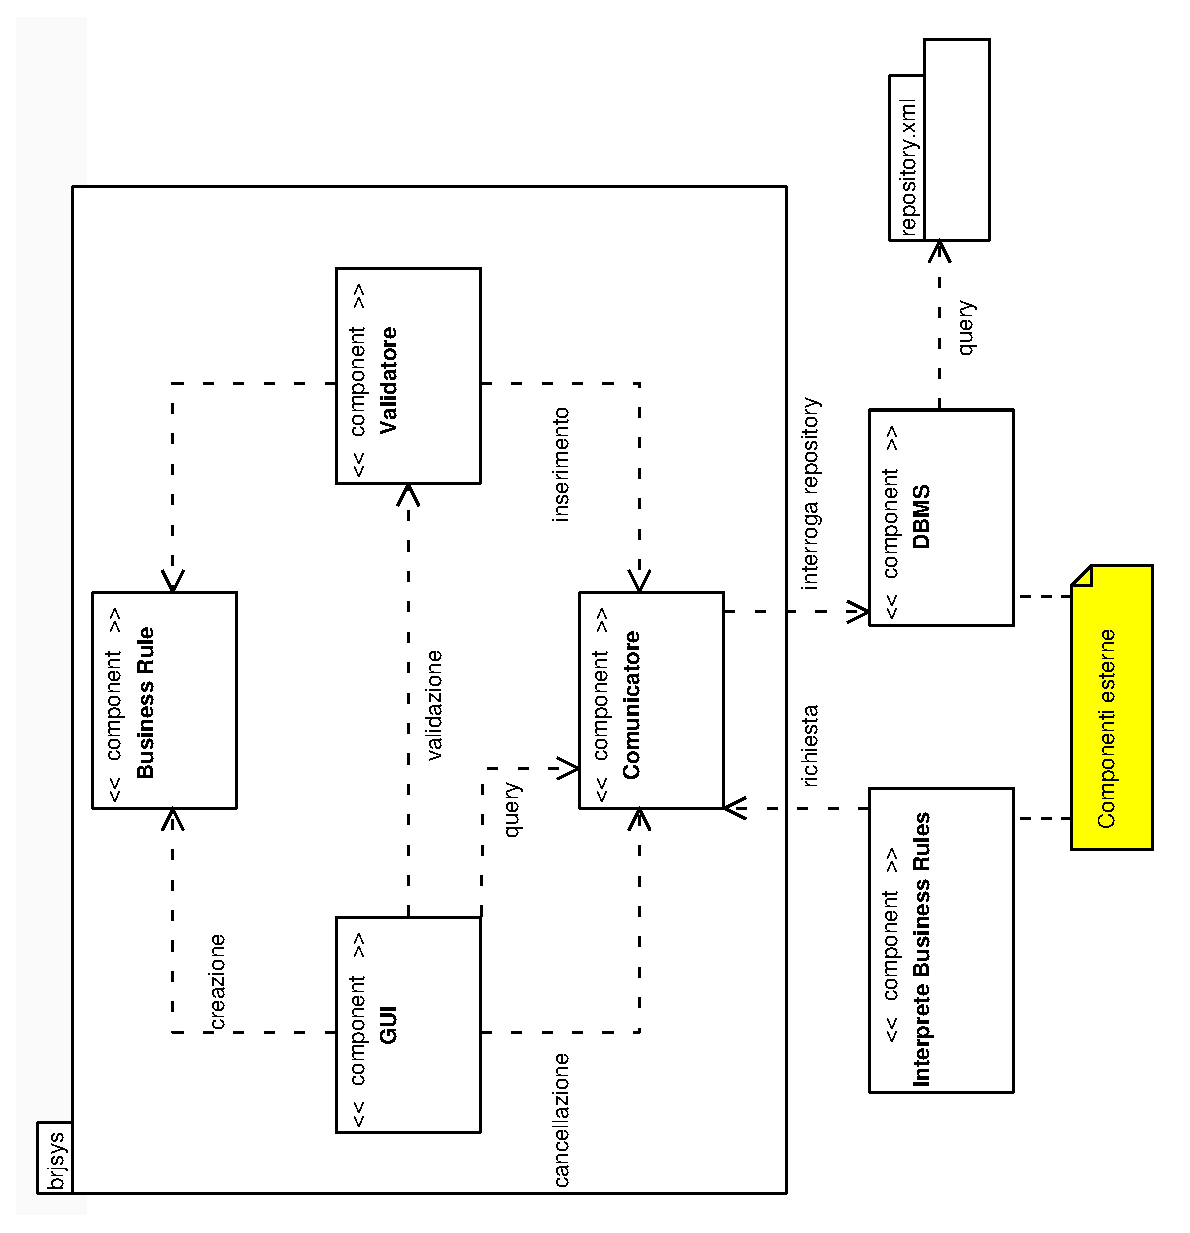
\includegraphics[width=0.8\textwidth, angle=-90]{class-dia/schemagenerale.eps}
\end{center}
Il prodotto \`e stato suddiviso in quattro macrocomponenti:
\begin{enumerate}
 \item \textbf{GUI}: Fornisce all'utente un interfaccia grafica minimale, consentendogli di effettuare operazioni di cancellazione e interrogazione del \re\ in maniera user-friendly.
\item \textbf{Business Rule}: Rappresenta la \br\ che l'utente dichiara e che deve essere passata al validatore per la compilazione.
\item \textbf{Validatore}: Accetta in input una \br, la valida e la inserisce, se scritta correttamente, nel \rp.
\item \textbf{Comunicatore}: Si connette al \underline{DBMS} esterno e comunica con esso tramite i formalismi del linguaggio \underline{XQuery}.
Sar\`a appunto tramite Query che il \underline{DBMS} effettuer\`a operazioni di inserimento, cancellazione o ricerca nel \rp, qualora un componente lo richieda.
\end{enumerate}
Questa suddivisione, per quanto minimale, consente di individuare le componenti che verranno poi ampliamente descritte nel successivo capitolo.

\chapter{Descrizione dei singoli componenti}
Analizzeremo qui le quattro macrocomponenti elencate in precedenza e ne daremo una descrizione pi\`u dettagliata.

\section{GUI}
\subsection{Diagramma delle classi}
\begin{center}
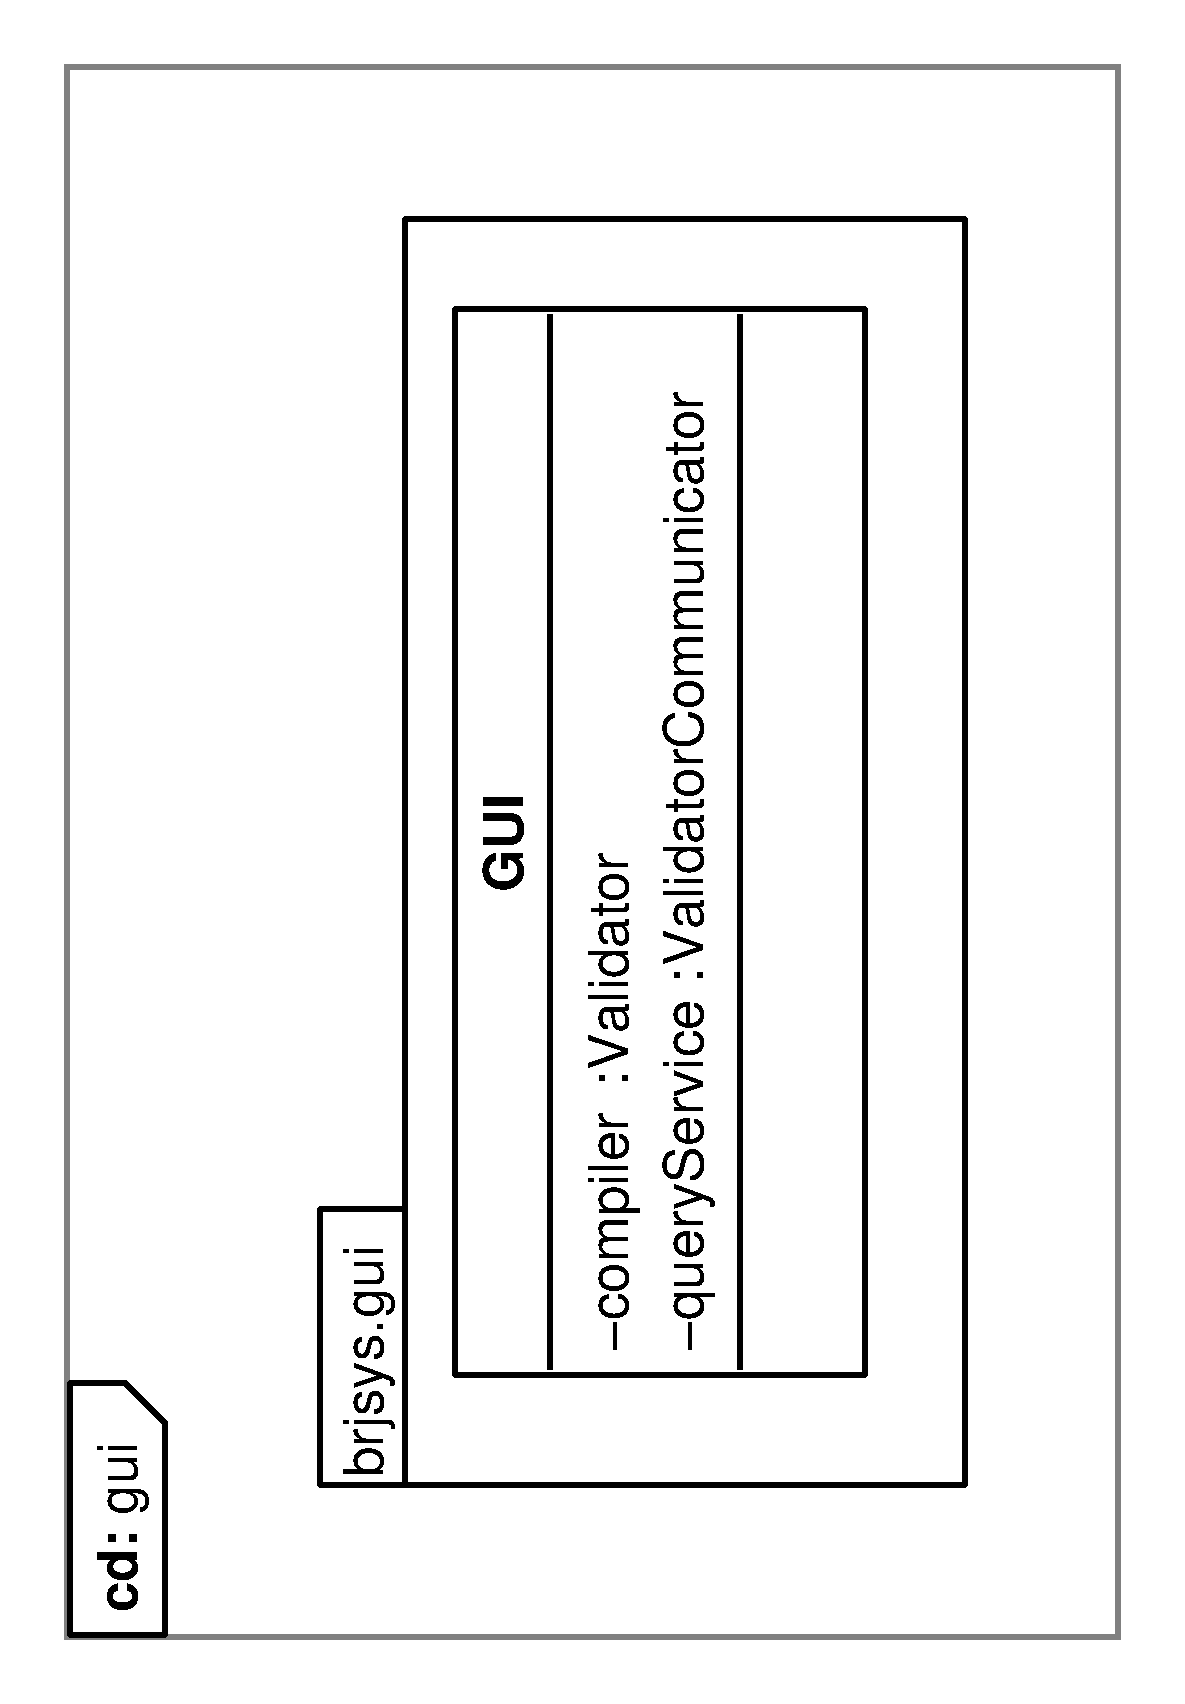
\includegraphics[width=0.3\textwidth, angle=-90]{class-dia/gui.eps}
\end{center}
\subsection{Gui}
%Diagramma della classe GUI...comprensivo di package
\subsubsection{Tipo, obiettivo e funzione del componente}
Questa componente, realizzata tramite una singola classe java, fornisce all'utente un'interfaccia minimale che gli consente di effettuare operazioni di cancellazione e querying sul \rp. Nel caso di esecuzione di una query definita dall'utente, verranno fornite anche informazioni relative ai tempi d'esecuzione.
\subsubsection{Relazioni d'uso di altre componenti}
Questa componente utilizza:
\begin{itemize}
 \item \BR\ per dichiarare una nuova \br\ da spedire al validatore;
 \item Validator per effettuare la validazione di una \br;
 \item GUICommunicator che verr\`a trattata successivamente.
\end{itemize}
\subsubsection{Interfacce con e relazioni di uso da altre componenti}
Nessuna.
\subsubsection{Attivit\`a svolte e dati trattati}
La componente Gui possiede i campi dato ``GUICommunicator'' e ``Validator'' che verranno utilizzati per fornire funzionalit\`a di interfacciamento. Tali funzionalit\`a verranno trattate in seguito.

\section{Validatore}
\subsection{Diagramma delle classi}
\begin{center}
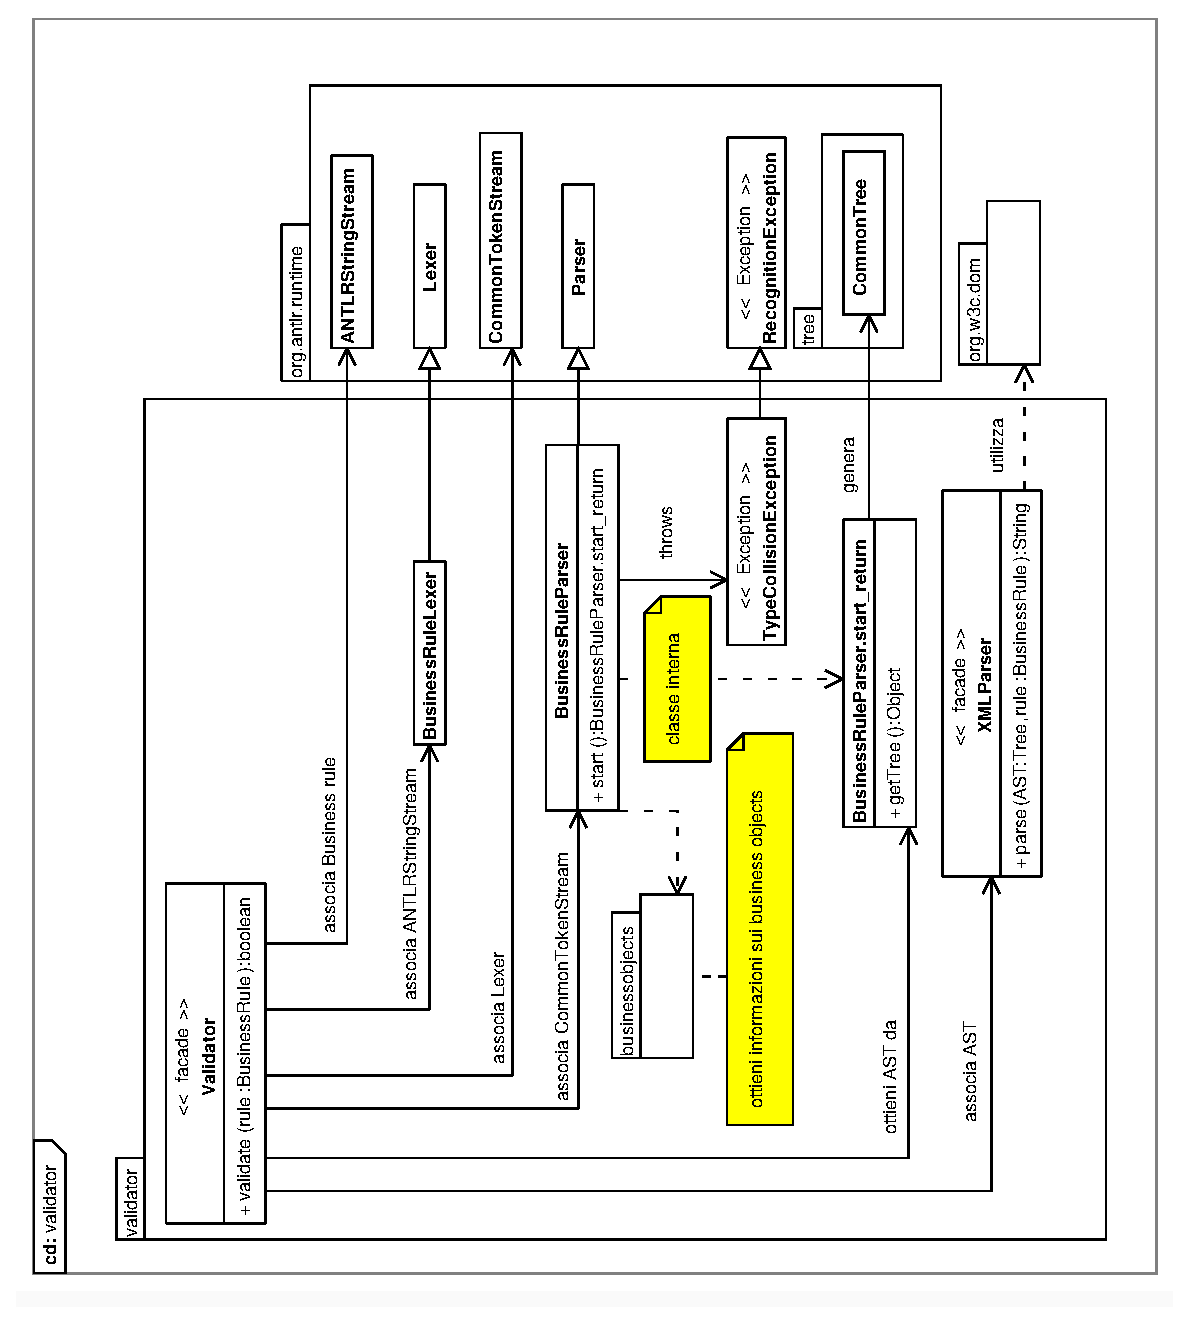
\includegraphics[width=0.6\textwidth, angle=-90]{class-dia/validator.eps}
\end{center}
\subsection{Validator}%facade!!!->va descritto
\subsubsection{Tipo, obiettivo e funzione del componente}
Questa componente effettua la validazione di una \br, dando la possibilit\`a all'utilizzatore di evitare le singole operazioni di compilazione. Ha il ruolo di \textit{fa\c{c}ade}: fornisce un'interfaccia unificata che riesce a gestire in maniera semplice ed immediata le operazioni di compilazione e inserimento che altrimenti dovremmo riportare direttamente dove la componente GUI lo richiedesse.
\subsubsection{Relazioni d'uso di altre componenti}
Validator usa le componenti \brp, \brl, XMLParser e ValidatorCommunicator. Quest'ultime verranno ampliamente descritte successivamente.
\subsubsection{Interfacce con e relazioni di uso da altre componenti}
La componente Validator \`e in relazione con la componente GUI, al fine di rendere possibile la validazione.
\subsubsection{Attivit\`a svolte e dati trattati}
Validator contiene solo il metodo validate(). Tale metodo effettua la validazione della \br.

\subsection{BusinessRuleLexer}
\subsubsection{Tipo, obiettivo e funzione del componente}
Questa componente, derivata da org.antlr.runtime.Lexer, non \`e altro che una classe \underline{wrapper} per la stringa che rappresenta la \br. Essa aggiunge funzionalit\`a alla stringa, necessarie per il successivo parsing.
\subsubsection{Relazioni d'uso di altre componenti}
Nessuna.
\subsubsection{Interfacce con e relazioni di uso da altre componenti}
La componente \brp\ necessita della componente \brl. Quest'ultima verr\`a approfondita in seguito.
\subsubsection{Attivit\`a svolte e dati trattati}
BusinessRuleLexer mette a disposizione vari metodi per la lettura del testo della \br, nonch\`e per la gestione di eventuali eccezioni avvenute in fase di validazione.\\
\textit{\textbf{Nota:}Questa classe \`e stata creata utilizzando uno strumento automatico per la generazione di parser data in input la specifica di una grammatica.}

\subsection{BusinessRuleParser}
\subsubsection{Tipo, obiettivo e funzione del componente}
Questa componente, derivata da org.antlr.runtime.Parser, effettua il parsing della stringa che rappresenta la \br. Effettua quindi il controllo sintattico della regola e il controllo semantico facendo un controllo sui tipi dei dati (siano essi costanti oppure campi dati di \bos). Mentre effettua la validazione, BusinessRuleParser genera l'albero di parsing secondo le specifiche presenti nel controllo semantico. \`E in grado infine di dare informazioni accurate riguardo eventuali errori in fase di validazione.
\subsubsection{Relazioni d'uso di altre componenti}
La componente BusinessRuleParser necessita di un \underline{token}Stream, fornitogli indirettamente da BusinessRuleLexer. Deve riferirsi poi alla componente BusinessObjects per effettuare il controllo sui tipi per il \bo\ associato. Per trattare gli errori in fase di validazione, ha bisogno infine della componente TypeCollisionException.
\subsubsection{Interfacce con e relazioni di uso da altre componenti}
\brp\ viene messa in relazione con XMLParser che verr\`a trattata successivamente.
\`E utilizzata inoltre dalla componente Validator.
\subsubsection{Attivit\`a svolte e dati trattati}
\brp\ mette a disposizione vari metodi per effettuare il parsing e i test semantici. Dispone inoltre di numerosi campi dato per la ricognizione dei \underline{token}.\\
\textit{\textbf{Nota:}Questa classe \`e stata creata utilizzando uno strumento automatico per la generazione di parser data in input la specifica di una grammatica.}

\subsection{TypeCollisionException}
\subsubsection{Tipo, obiettivo e funzione del componente}
Questa componente, derivata dalla classe\\ org.antlr.runtime.RecognitionException, permette di ricavare informazioni sugli eventuali errori avvenuti in fase di parsing della \br. In definitiva aggiunge alla sua superclasse la possibilit\`a di riportare informazioni su errori di tipo.
\subsubsection{Relazioni d'uso di altre componenti}
Nessuna.
\subsubsection{Interfacce con e relazioni di uso da altre componenti}
La componente TypeCollisionException \`e utilizzata da \brp\ per sollevare eccezioni derivanti da errori di tipo.
\subsubsection{Attivit\`a svolte e dati trattati}
Viene ridefinito il metodo printStackTrace() e messo a disposizione un costruttore per avere informazioni sui tipi che si sono rivelati incompatibili.

\subsection{XMLParser}%probabilmente è un facade anche questo
\subsubsection{Tipo, obiettivo e funzione del componente}
La componente XMLParser si occupa di effettuare la conversione dell'albero sintattico prodotto dalla componente \brp\ in un elemento XML rappresentante la \br. L'elemento XML risultante conterr\`a:
\begin{itemize}
 \item il nome della \br, che dovr\`a essere univoco;
 \item il nome del \bo\ associato alla regola;
 \item la struttura dell'\underline{AST} della \br, scritta secondo la metodologia elemento-attributo tipica di XML;
 \item la struttura dell'\underline{AST} della \br, scritta linearmente secondo la notazione prefissa rappresentata da un singolo attributo XML;
 \item la \br\ effettivamente digitata dall'utente;
 \item eventuali commenti associati dall'utente alla \br.
\end{itemize}
XMLParser ha in questo contesto il ruolo del design pattern \textit{fa\c{c}ade}. La creazione di un elemento XML tramite il package java \textit{org.w3c.dom} necessita di operazioni sequenziali che coinvolgono numerose classi e numerosi metodi. Implementare tutte queste procedure direttamente nella classe Validator renderebbe il codice meno leggibile e meno manipolabile.
\subsubsection{Relazioni d'uso di altre componenti}
XMLParser ha bisogno dell'\underline{AST} prodotto da \brp, nonch\`e  della componente \br\ per ricavare le informazioni da inserire nell'elemento XML.
\subsubsection{Interfacce con e relazioni di uso da altre componenti}
La componente ValidatorCommunicator necessita dell'elemento XML prodotto da XMLParser per avviare la procedura di inserimento nel \rp.
\subsubsection{Attivit\`a svolte e dati trattati}
XMLParser contiene le operazioni per scorrere l'\underline{AST} ed effettuare la traduzione in XML.

\subsection{businessobjects}%è un package
\subsubsection{Tipo, obiettivo e funzione del componente}
La componente businessobjects si occupa di offrire un namespace comune a tutti i \bos\ che durante la validazione di una \br\ vengono interpellati richiedendo accesso ai relativi campi dato o sottocampi dato.
\subsubsection{Relazioni d'uso di altre componenti}
Nessuna.
\subsubsection{Interfacce con e relazioni di uso da altre componenti}
\brp necessita di questa componente per effettuare il controllo dei tipi qualora fosse necessario.
\subsubsection{Attivit\`a svolte e dati trattati}
La componente businessbjects offre al validatore le classi java che rappresentano i \bos.

\section{Business Rule}
\subsection{Diagramma delle classi}
\begin{center}
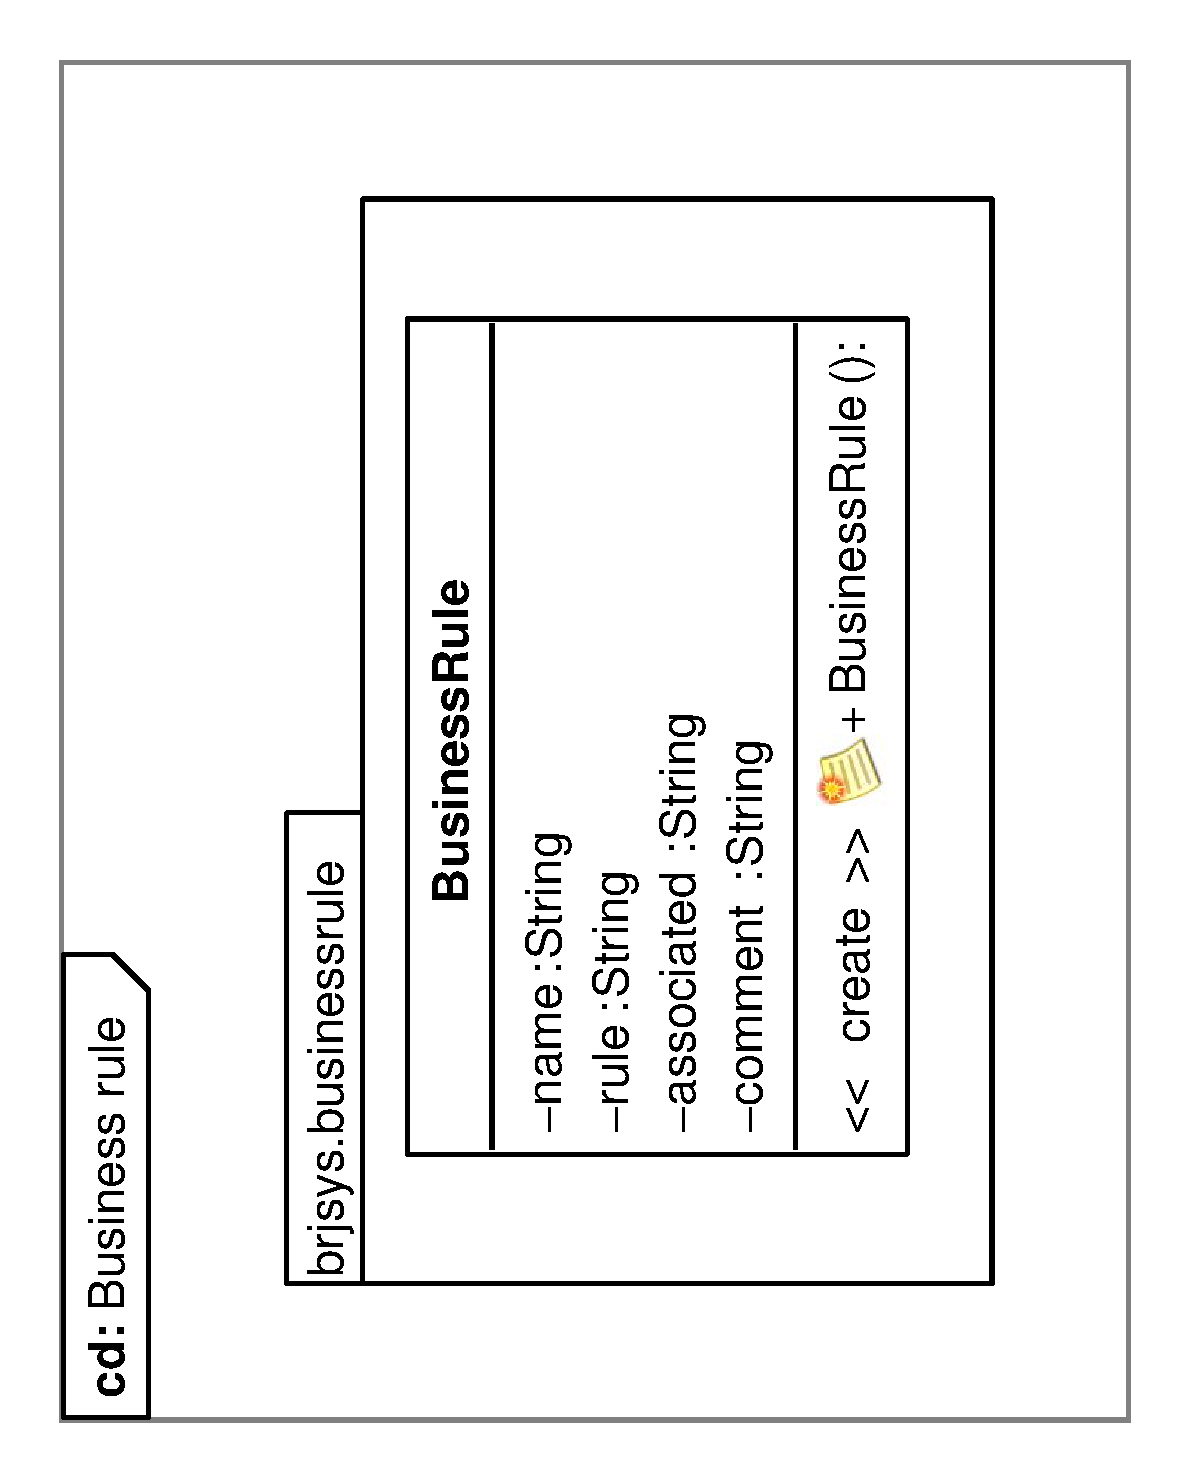
\includegraphics[width=0.3\textwidth, angle=-90]{class-dia/Businessrule.eps}
\end{center}
\subsection{BusinessRule}
\subsubsection{Tipo, obiettivo e funzione del componente}
La componente \BR\ rappresenta la \br\ che l'utente inserisce e vuole validare.
\subsubsection{Relazioni d'uso di altre componenti}
Nessuna.
\subsubsection{Interfacce con e relazioni di uso da altre componenti}
La componente GUI utilizza \BR\ nel caso in cui l'utente voglia inserire una nuova \br.
La componente Validator effettua la validazione di un'istanza di \BR, tramite la chiamata del suo metodo validate().
\subsubsection{Attivit\`a svolte e dati trattati}
Business Rule contiene i campi dato Stringa per rappesentare una \br\ (name, associatedObject, rule e comment, dove quest'ultimo pu\`o anche non essere istanziato). Vengono messi inoltre a disposizione il costruttore e il metodo ridefinito toString().

\section{Comunicatore}
\subsection{Diagramma delle classi}
\begin{center}
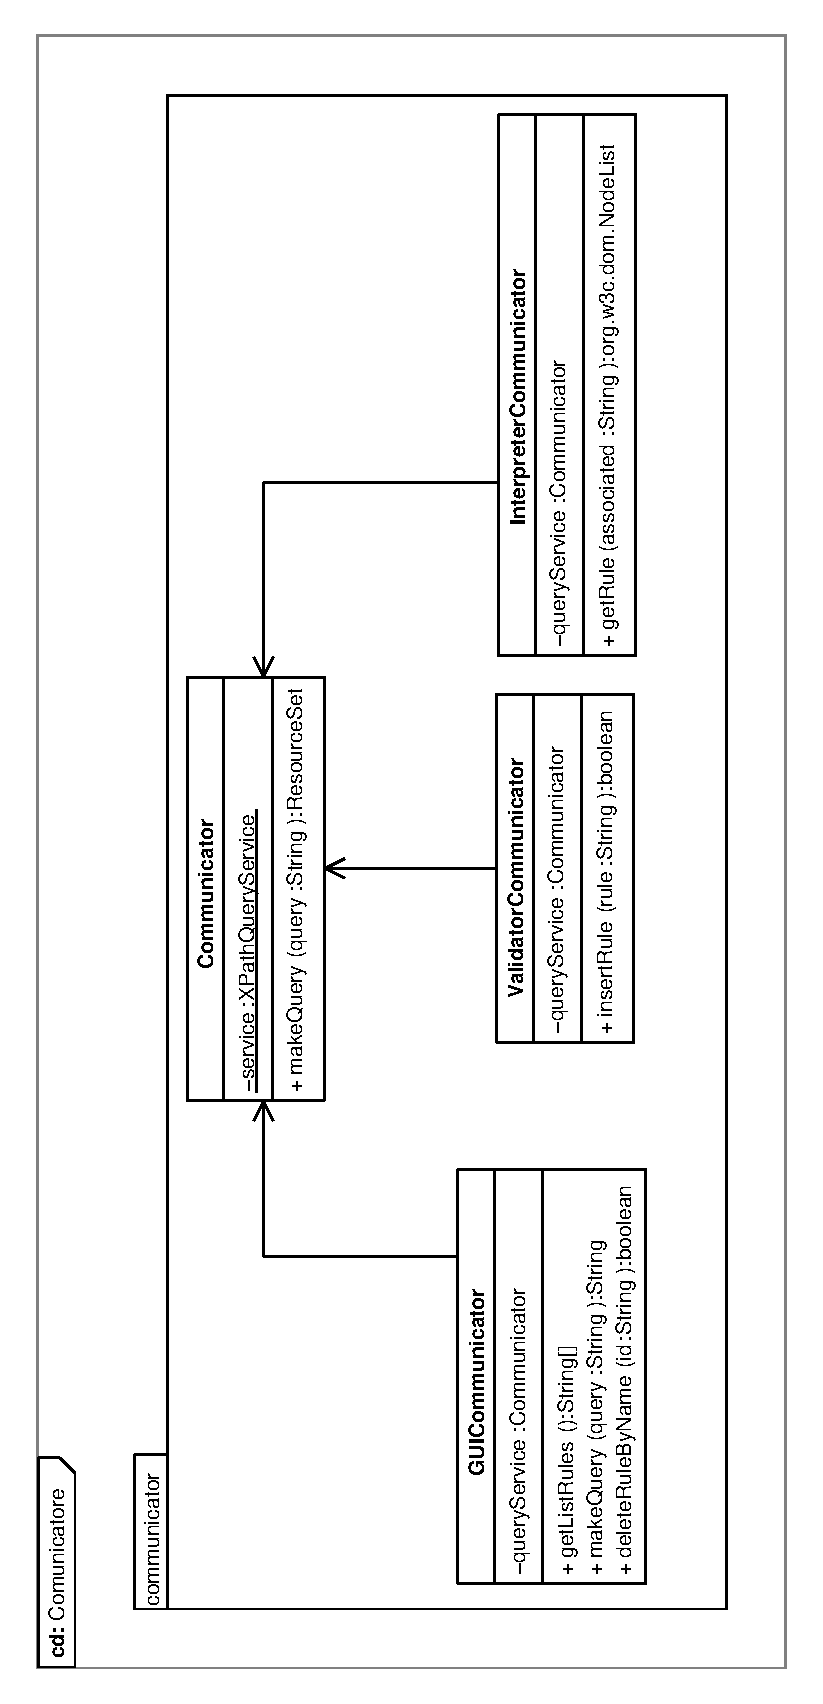
\includegraphics[width=0.4\textwidth, angle=-90]{class-dia/Comunicatore.eps}
\end{center}
\subsection{Communicator}
\subsubsection{Tipo, obiettivo e funzione del componente}
La componente Communicator fornisce alle componenti che la utilizzano la possibilit\`a di effettuare query di qualsiasi tipo al \rp\ presente nel \underline{DBMS}.
\subsubsection{Relazioni d'uso di altre componenti}
Communicator necessita di interagire con la componente esterna \underline{DBMS} per interrogare il \rp.
\subsubsection{Interfacce con e relazioni di uso da altre componenti}
Le componenti GUICommunicator, InterpreterCommunicator e ValidatorCommunicator necessitano di Communicator per potergli passare query specifiche. Le loro descrizioni verranno trattate successivamente.
\subsubsection{Attivit\`a svolte e dati trattati}
Quando viene istanziata per la prima volta, Communicator inizializza la connessione al \underline{DBMS} tramite la definizione di una variabile statica. Consente successivamente di interrogare il \rp\ direttamente, passandogli la stringa che rappresenta la query composta secondo le specifiche \underline{XQuery}.
%
\subsection{GUICommunicator}
\subsubsection{Tipo, obiettivo e funzione del componente}
La componente GUICommunicator contiene metodi necessari per modellare query di cancellazione (tramite operazioni \underline{XQuery} Update) e query di semplice interrogazione.
\subsubsection{Relazioni d'uso di altre componenti}
GUICommunicator utilizza la componente Communicator per accedere al \rp\ ed interrogarlo.
\subsubsection{Interfacce con e relazioni di uso da altre componenti}
GUICommunicator viene messa in relazione con la componente GUI, dalla quale riceve richieste di cancellazione e di querying.
\subsubsection{Attivit\`a svolte e dati trattati}
La componente fornisce le seguenti operazioni:
\begin{itemize}
 \item deleteRuleByName(): dato il nome di una regola, provvede ad eliminarla dal \rp\ nel caso questa regola sia presente;
 \item makeQuery(): permette l'esecuzione di una semplice query purch\`e non implichi modifiche strutturali al \rp;
 \item getListRules(): ritorna per ogni \br, nome, \bo\ associato e struttura.
\end{itemize}
\subsection{InterpreterCommunicator}
\subsubsection{Tipo, obiettivo e funzione del componente}
La componente InterpreterCommunicator contiene metodi necessari per rispondere a richieste di \br\ da parte di un interprete esterno.
\subsubsection{Relazioni d'uso di altre componenti}
InterpreterCommunicator utilizza la componente Communicator per accedere al \rp\ ed interrogarlo.
\subsubsection{Interfacce con e relazioni di uso da altre componenti}
InterpreterCommunicator viene messa in relazione con l'interprete esterno, dal quale riceve richieste di \brs\ associate ad un determinato \bo.
\subsubsection{Attivit\`a svolte e dati trattati}
La componente InterpreterCommunicator offre il metodo getRule() per richiedere le \br\ associate al \bo.

\subsection{ValidatorCommunicator}
\subsubsection{Tipo, obiettivo e funzione del componente}
La componente ValidatorCommunicator contiene metodi necessari per effettuare l'inserimento di una \br\ validata gi\`a tradotta in XML.
\subsubsection{Relazioni d'uso di altre componenti}
ValidatorCommunicator utilizza la componente Communicator per accedere al \rp\ ed interrogarlo.
\subsubsection{Interfacce con e relazioni di uso da altre componenti}
ValidatorCommunicator viene messa in relazione con la componente Validator per effettuare l'inserimento.
\subsubsection{Attivit\`a svolte e dati trattati}
La componente offre il metodo insertRule() per inserire la \br\ nel \rp. L'inserimento avverr\`a soltanto se la \br\ ha un nome che non \`e ancora presente nel \rp.

\chapter{Componenti esterne}
\begin{center}
 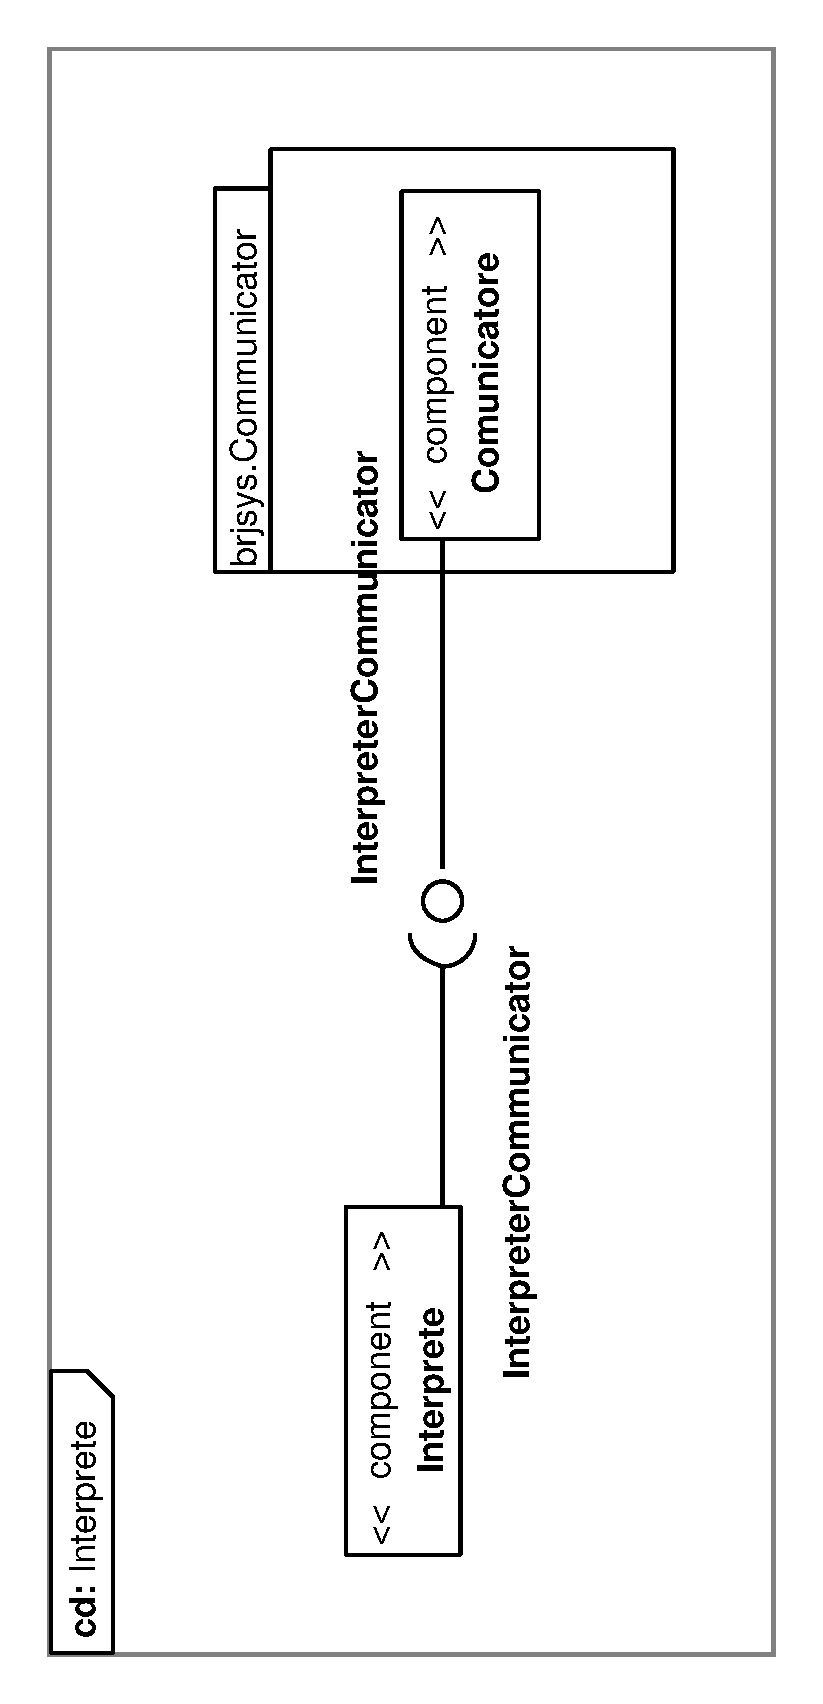
\includegraphics[width=0.4\textwidth, angle=-90]{class-dia/Interprete.eps}
\end{center}
\section{Interprete}
\subsubsection{Tipo, obiettivo e funzione del componente}
Questo componente si incarica di eseguire le \brs\ associate ad un determinato \bo. Per ottenere le \br, deve poter interrogare il \underline{DBMS} attraverso un opportuna interfaccia col sistema \underline{BR-jsys} che risolver\`a per lui la richiesta.
\subsubsection{Relazioni d'uso di altre componenti}
La componente Interprete utilizza la componente InterpreterCommunicator per comunicare col \underline{DBMS}.
\subsubsection{Interfacce con e relazioni di uso da altre componenti}
Nessuna.
\subsubsection{Attivit\`a svolte e dati trattati}
Non siamo tenuti a considerare i dettagli riguardanti le operazioni specifiche della componente. L'unico vincolo posto \`e che comunichi con il \underline{DBMS} tramite l'interfaccia InterpreterCommunicator.
\section{\underline{DBMS}}
\begin{center}
 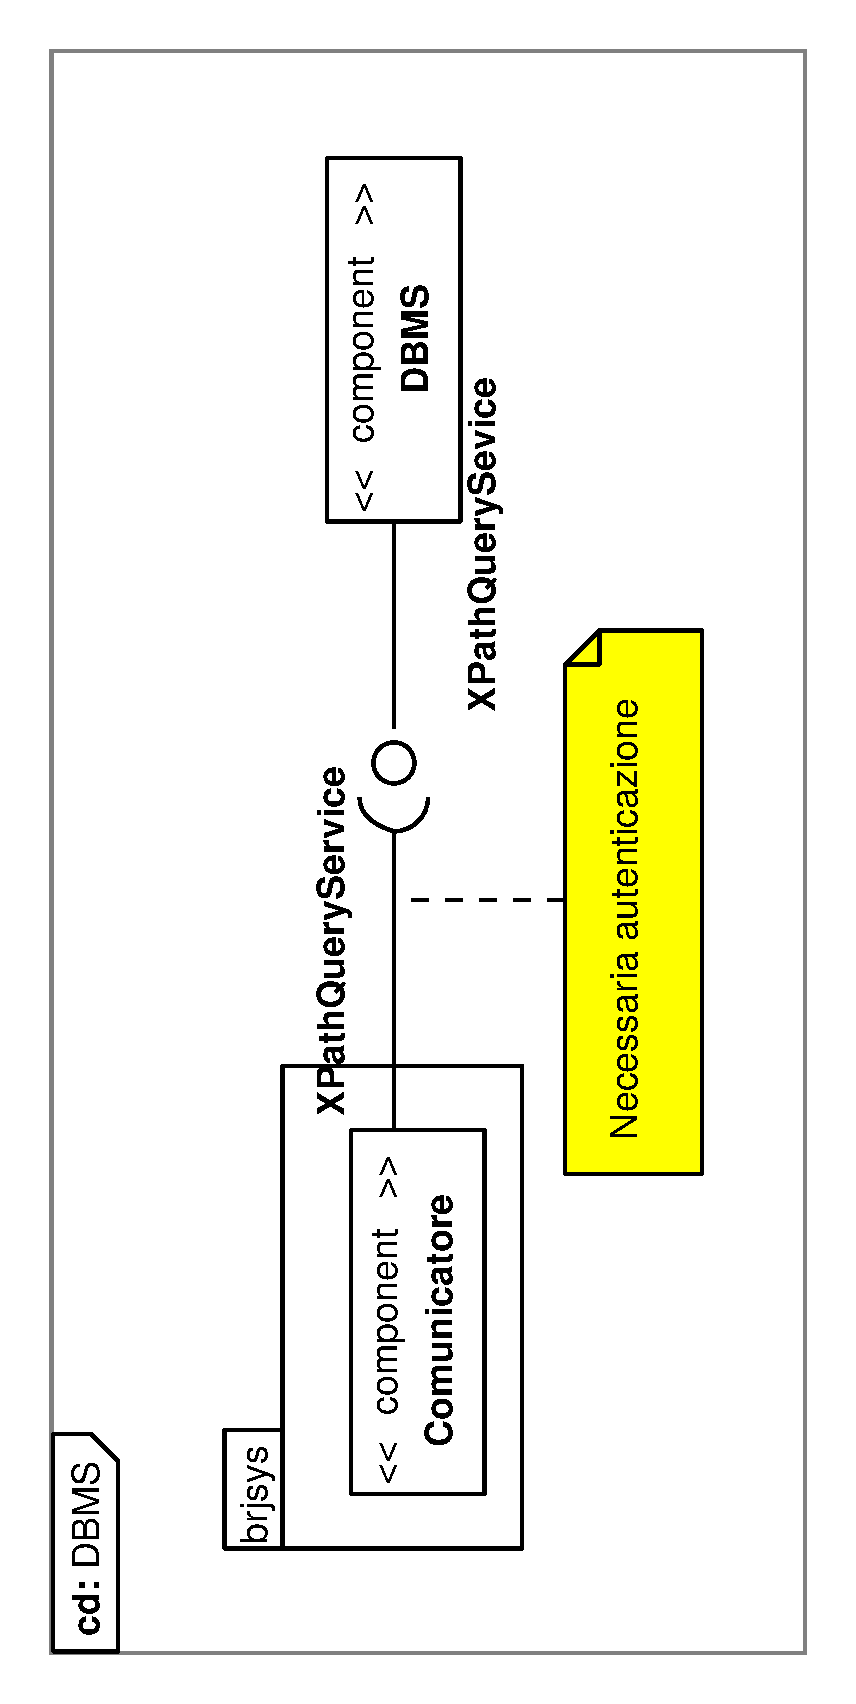
\includegraphics[width=0.5\textwidth, angle=-90]{class-dia/DBMS.eps}
\end{center}
\subsubsection{Tipo, obiettivo e funzione del componente}
Questa componente serve a comunicare con il \rp\ in modo efficiente. La comunicazione avverr\`a tramite linguaggio \underline{XQuery}.
\subsubsection{Relazioni d'uso di altre componenti}
Nessuna.
\subsubsection{Interfacce con e relazioni di uso da altre componenti}
Previa una connessione corretta, il \underline{DBMS} mette a disposizione un'interfaccia XPathQueryService con la quale interagire col \rp\ presente all'interno del \underline{DBMS} stesso.
\subsubsection{Attivit\`a svolte e dati trattati}
Una corretta autenticazione far\`a in modo che l'interfaccia di tipo XPathQueryService possa interagire col \rp\ tramite il metodo query(). Quest'ultimo accetta come parametro una query impostata secondo le specifiche \underline{XQuery}.

\chapter{Diagrammi}
\section{Diagrammi di attivit\`a}

\subsection{Richiesta dell'interprete}
\begin{center}
 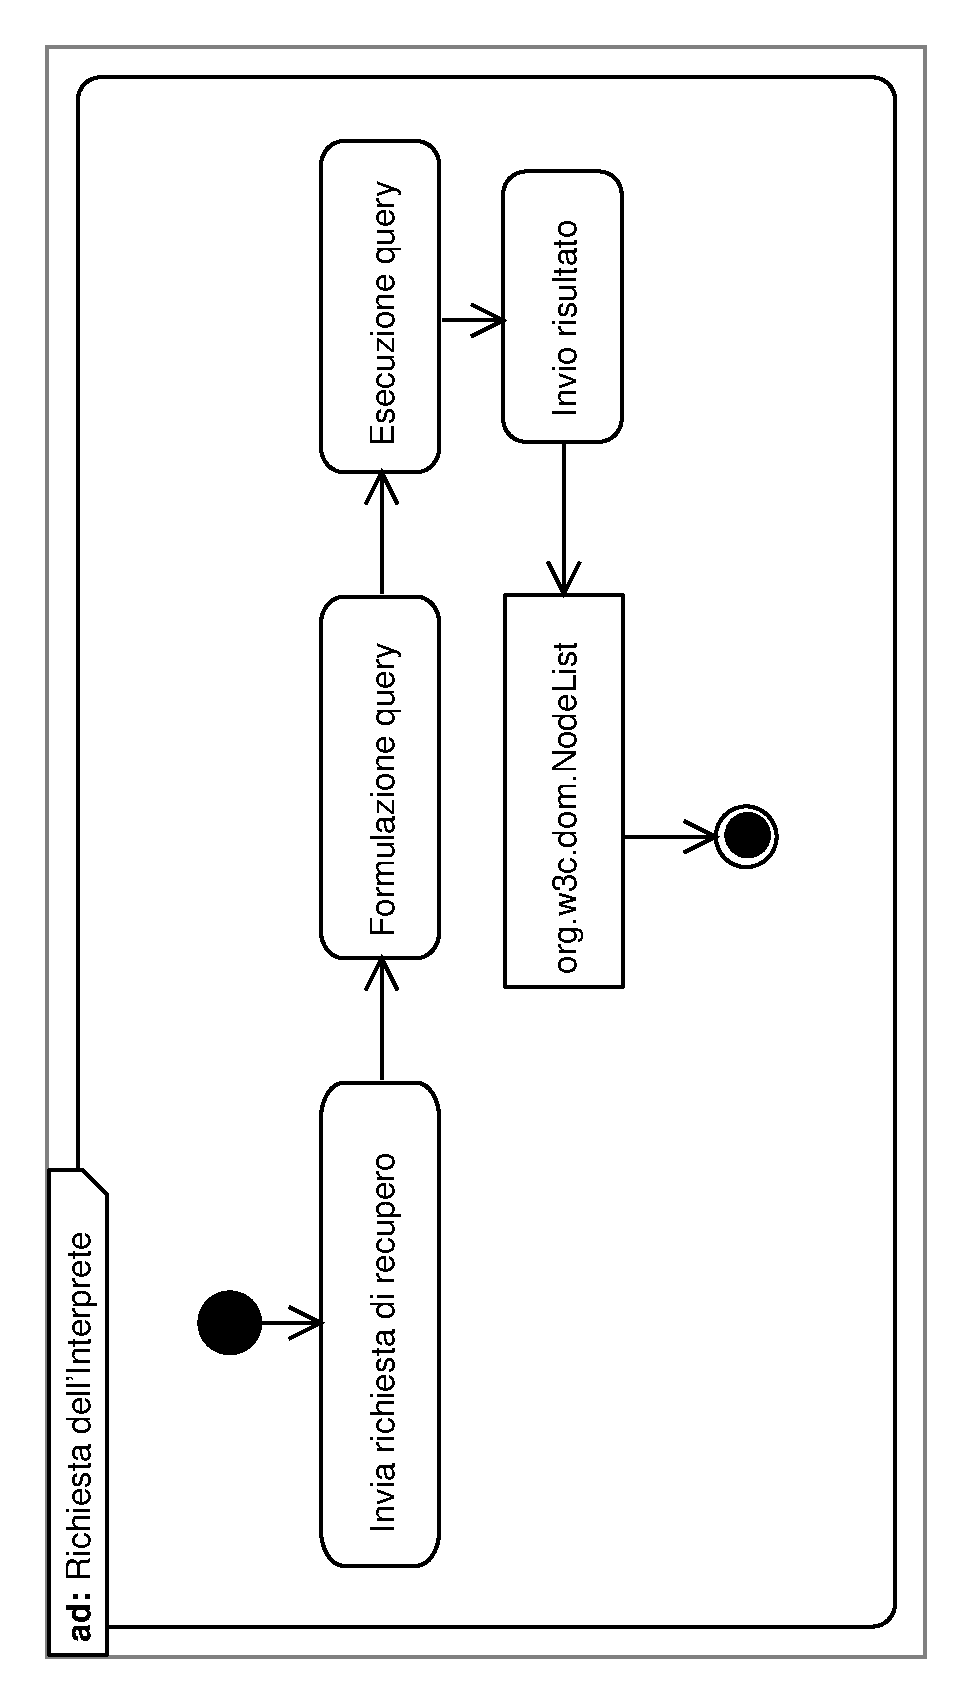
\includegraphics[width=0.5\textwidth, angle=-90]{activity-dia/RichiestadellInterprete.eps}
\end{center}
L'interprete invia la richiesta al sistema, il quale formula la query da inviare al \underline{DBMS}. La query viene quindi eseguita e il risultato viene tornato all'interprete sottoforma di un oggetto \textit{org.w3c.dom.NodeList}.

\subsection{GUI}
\begin{center}
 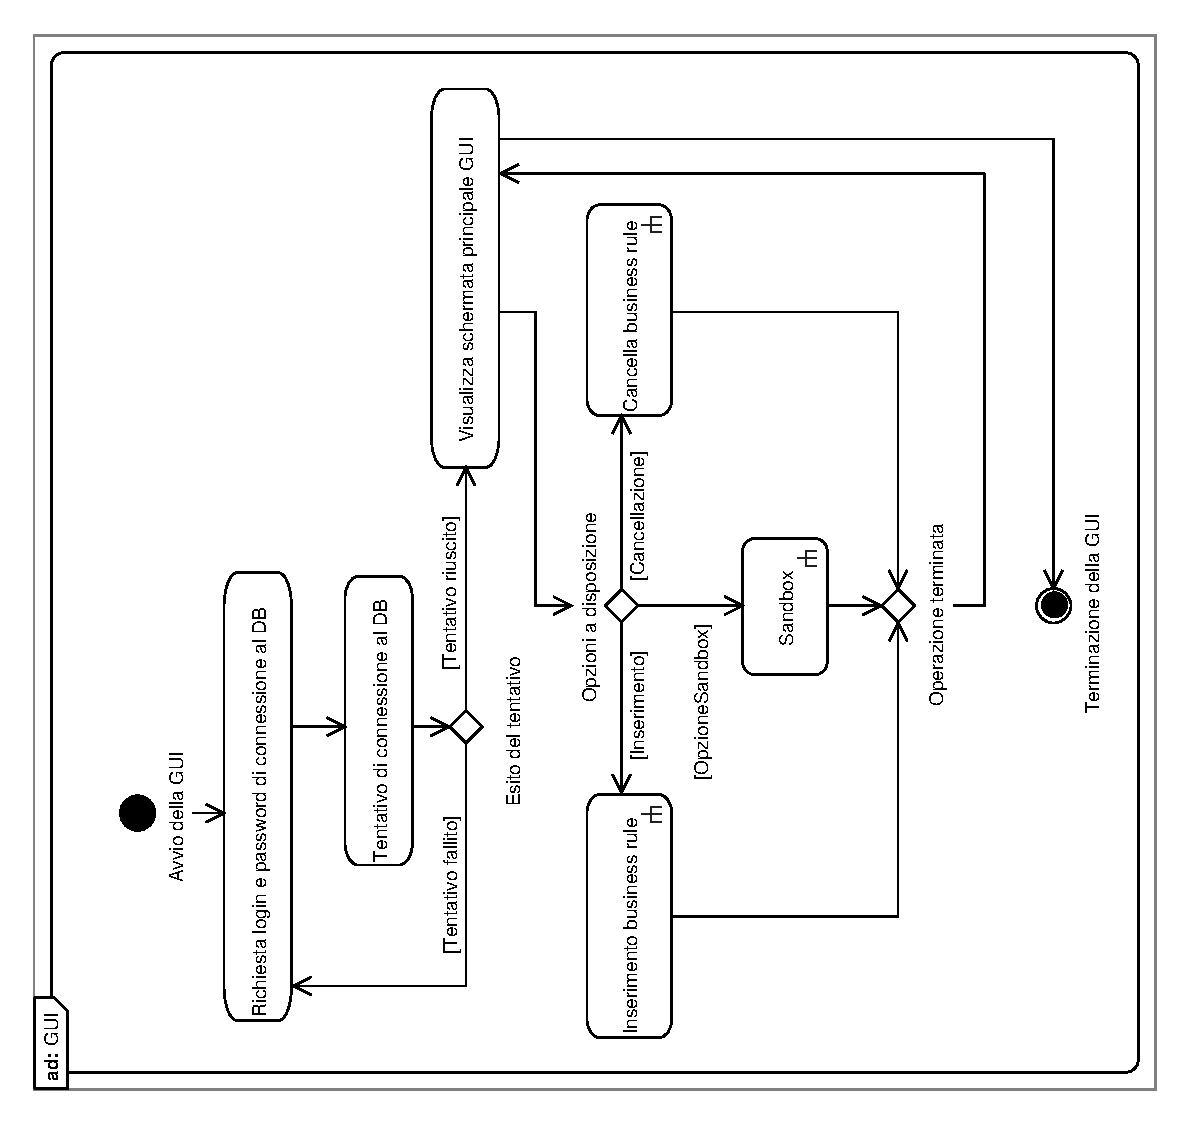
\includegraphics[width=1\textwidth, angle=-90]{activity-dia/GUI.eps}
\end{center}
All'avvio della GUI viene visualizzato un messaggio in cui vengono richiesti \textit{login} e \textit{password}. Si cerca quindi di stabilire una connessione qualificata al DB. 
Si controlla quindi l'esito del tentativo di connessione; se il tentativo ha dato esito negativo si richiede la \textit{login} e la
 \textit{password} all'utente. Se, al contrario, l'esito \`e positivo, ossia si ha disposizione una connessione, viene visualizzata la schermata della GUI dalla quale  possono essere lanciati :\textit{ l'inserimento di una \br}, \textit{l'avvio di una \underline{Sandbox}}, \textit{la cancellazione di una \br}.
Nel diagramma queste tre attivit\`a sono rappresentate come delle \textit{sub-activity} che vengono illustrate di seguito. Al termine di ogni operazione l'utente viene riportato alla finestra principale dove pu\`o effettuare una nuova operazione oppure terminare l'esecuzione della GUI stessa.

\subsection{Inserisci \br}
\begin{center}
 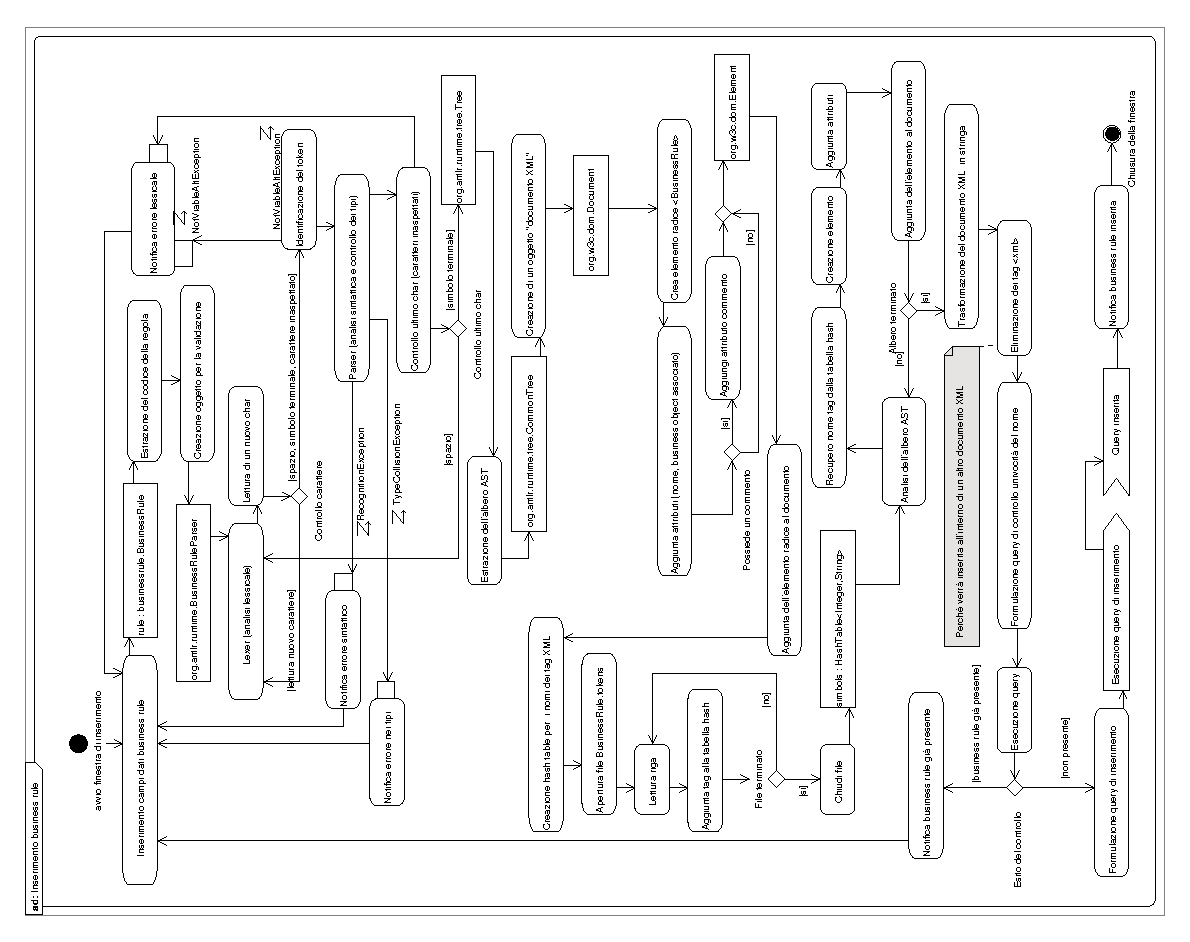
\includegraphics[width=1.1\textwidth, angle=-90]{activity-dia/InserisciBusinessRule.eps}
\end{center}

Una volta avviata la finestra di inserimento l'utente inserir\`a i campi dato per la \br\, verr\`a dunque costruito un oggetto \textit{\BR\ }. Quest'oggetto verr\`a inviato al parser che lo convertir\`a in un \underline{AST} dopo aver controllato la validit\`a della regola (Vedi diagramma Conversione \br -\underline{AST}), se la regola mostra errori verr\`a sollevata una eccezione, altrimenti si passer\`a alla fase di conversione da \underline{AST} a stringa rappresentante un elemento XML (Vedi diagramma Conversione \underline{AST}-XML). La fase successiva sar\`a quella di inserire la regola nel \rp\ (Vedi Diagramma Inserimento \br\ nel \rp). In caso di esito positivo dell'inserimento si dovr\`a uscire dalla finestra inserimento, altrimenti si informer\`a l'utente del errore e si ritorner\`a alla finestra iniziale.

\subsubsection{Conversione \br -\underline{AST}}
\begin{center}
 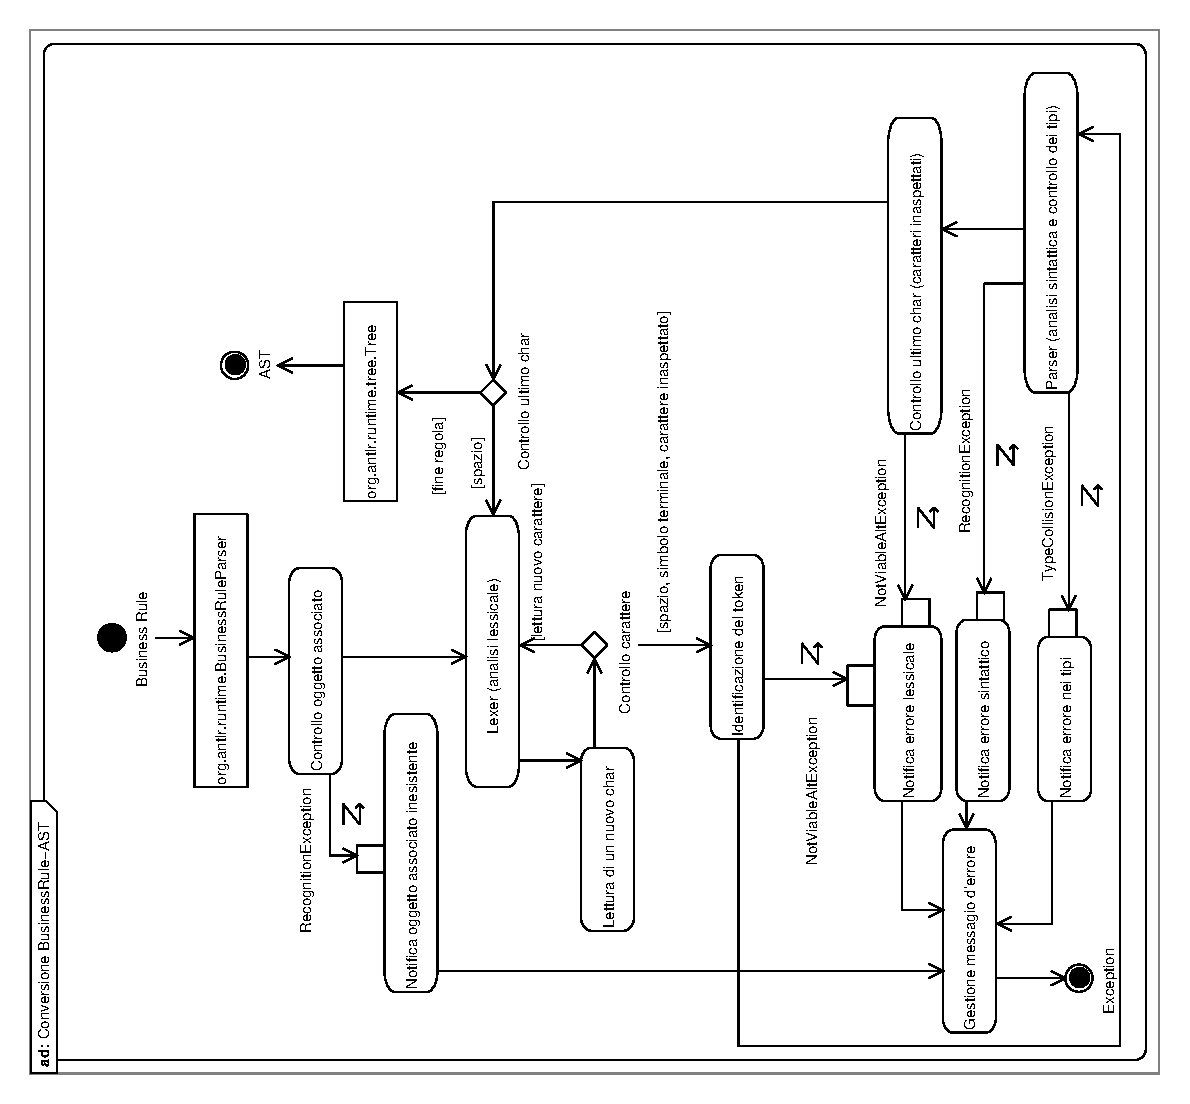
\includegraphics[width=1\textwidth, angle=-90]{activity-dia/ConversioneBusinessRuleAST.eps}
\end{center}
Al parser arriva in ingresso una stringa rappresentante la \br\ da validare. Inizialmente si controller\`a che la \br\ si riferisca ad un \bo\ valido, in caso contrario la validazione verr\`a subito bloccata. Dopodich\`e verranno fatti vari controlli con lo scopo di scorrere tutta la regola alla ricerca di errori sintattici, lessicali o logici, nel caso venissero trovati verranno invocate le opportune eccezioni che verranno gestite in maniera da ritornare al chiamante la struttura dell'errore che ne indicher\`a il tipo e la posizione nella \br\ dove \`e avvenuto. In caso di validazione senza errori verr\`a generato un opportuno \underline{AST} che successivamente si convertir\`a 
in una stringa in XML.


\subsubsection{Conversione \underline{AST}-XML}
\begin{center}
 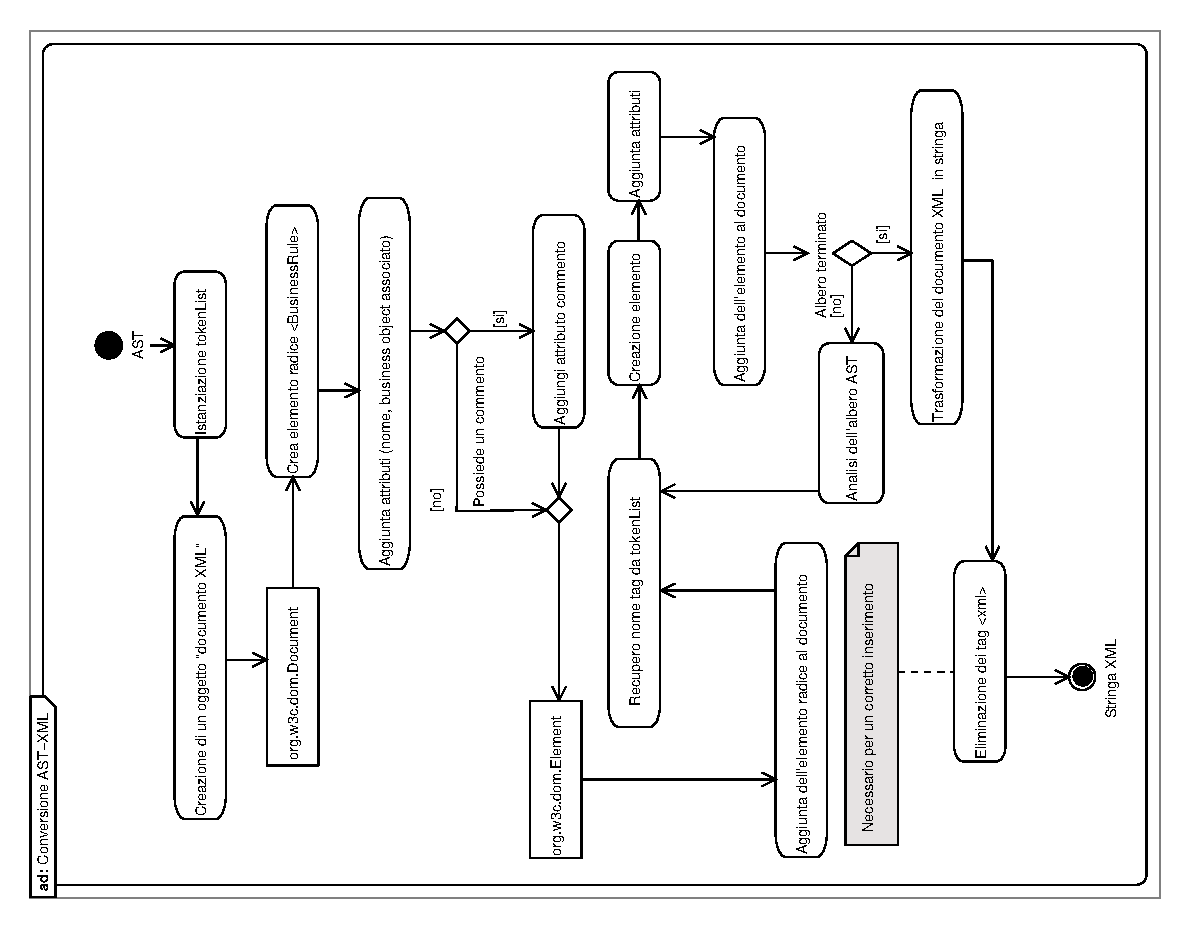
\includegraphics[width=1\textwidth, angle=-90]{activity-dia/ConversioneASTXML.eps}
\end{center}
Abbiamo ora a disposizione un \underline{AST} che dovremo scorrere in maniera prefissa per generare l'elemento XML da inserire nel \rp. Innanzi tutto abbiamo bisogno di sapere come il parser identifica (tramite un numero intero univoco) i vari \underline{token}. La struttura non \`e altro che un array che associa un intero univoco al \underline{token} della grammatica. Dopodich\`e si seguir\`a la prassi tipica del package \textit{org.w3c.dom} per la generazione di un elemento XML. Il L'elemento radice della \br\ scritta in XML conterr\`a il nome della regola, il \bo\ associato, il testo della regola e l'eventuale commento.
Si scorrer\`a ricorsivamente l'\underline{AST} percorrendo tutti i nodi aggiornando la struttura dell'elemento XML. Una volta completata la scansione e la relativa generazione dell'elemento XML lo si dovr\`a convertire in stringa, infine si dovr\`a rimuovere l'intestazione che di consuetudine si trova in tutti i documenti XML (esempio \textit{\textless?xml version="1.0" encoding="UTF-8"?\textgreater}) che impedirebbe l'inserimento nel \rp\ tramite query.

\subsubsection{Inserimento \br\ nel \rp}
\begin{center} 
 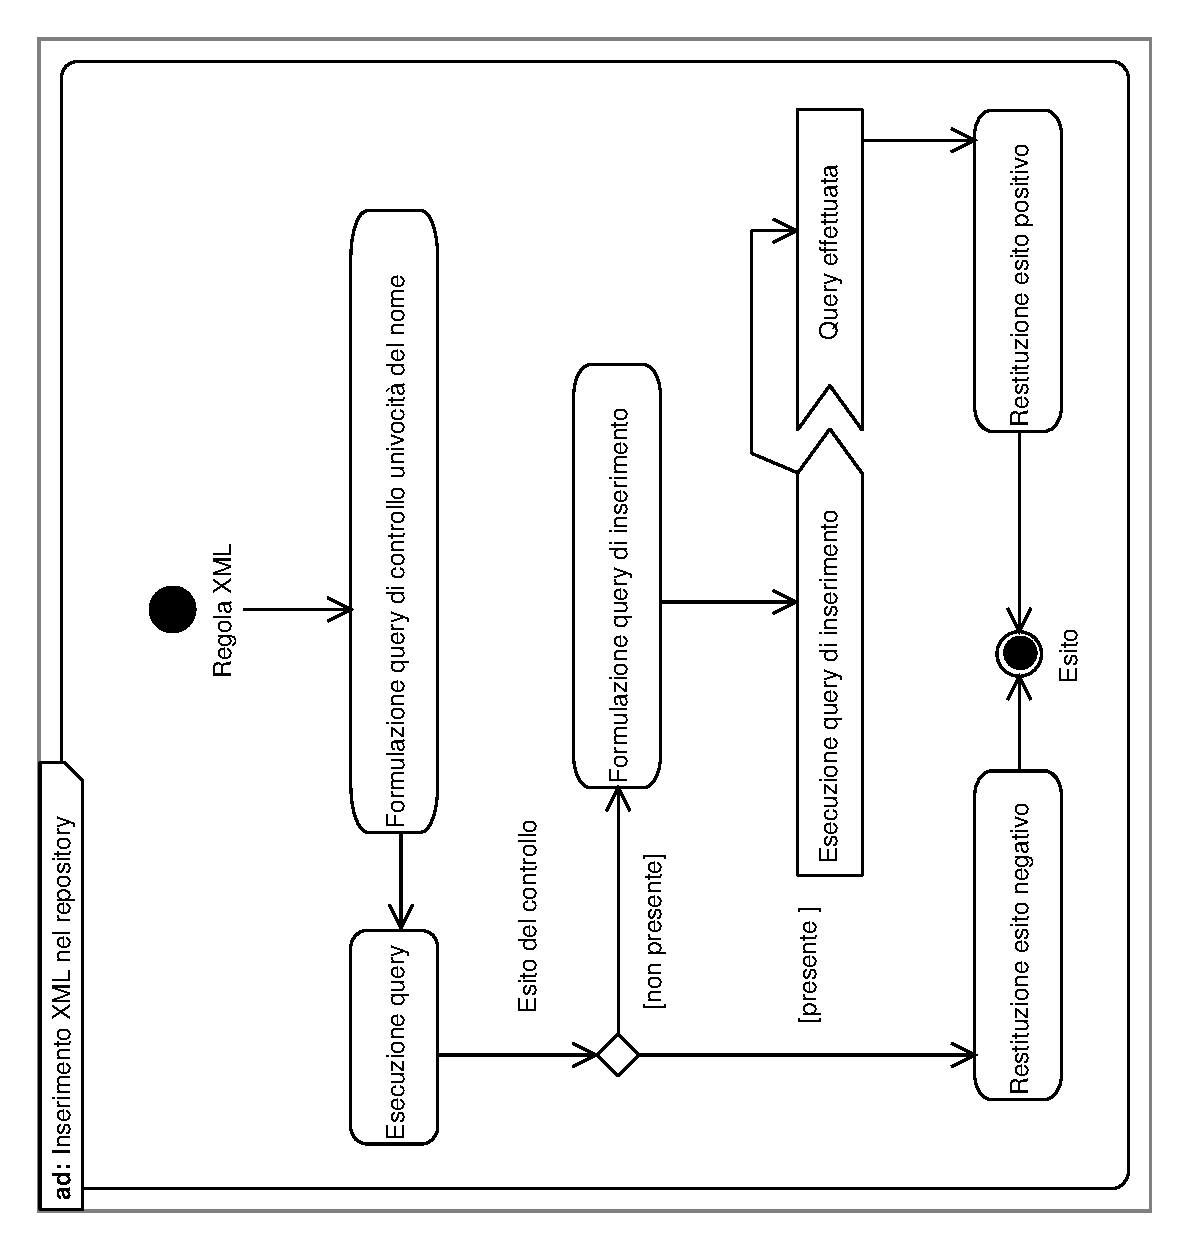
\includegraphics[width=0.9\textwidth, angle=-90]{activity-dia/InserimentoXMLnelrepository.eps}
\end{center}
Si dovr\`a prima di tutto controllare che il nome della regola si vuole inserire non sia gi\`a presente nel \rp. Se \`e gi\`a presente si troncher\`a immediatamente l'operazione di inserimento, altrimenti sar\`a formulata la query adatta per inserire la \br\ e si indicher\`a al chiamante che l'operazione \`e riuscita con successo.

\subsection{Sandbox}
\begin{center}
 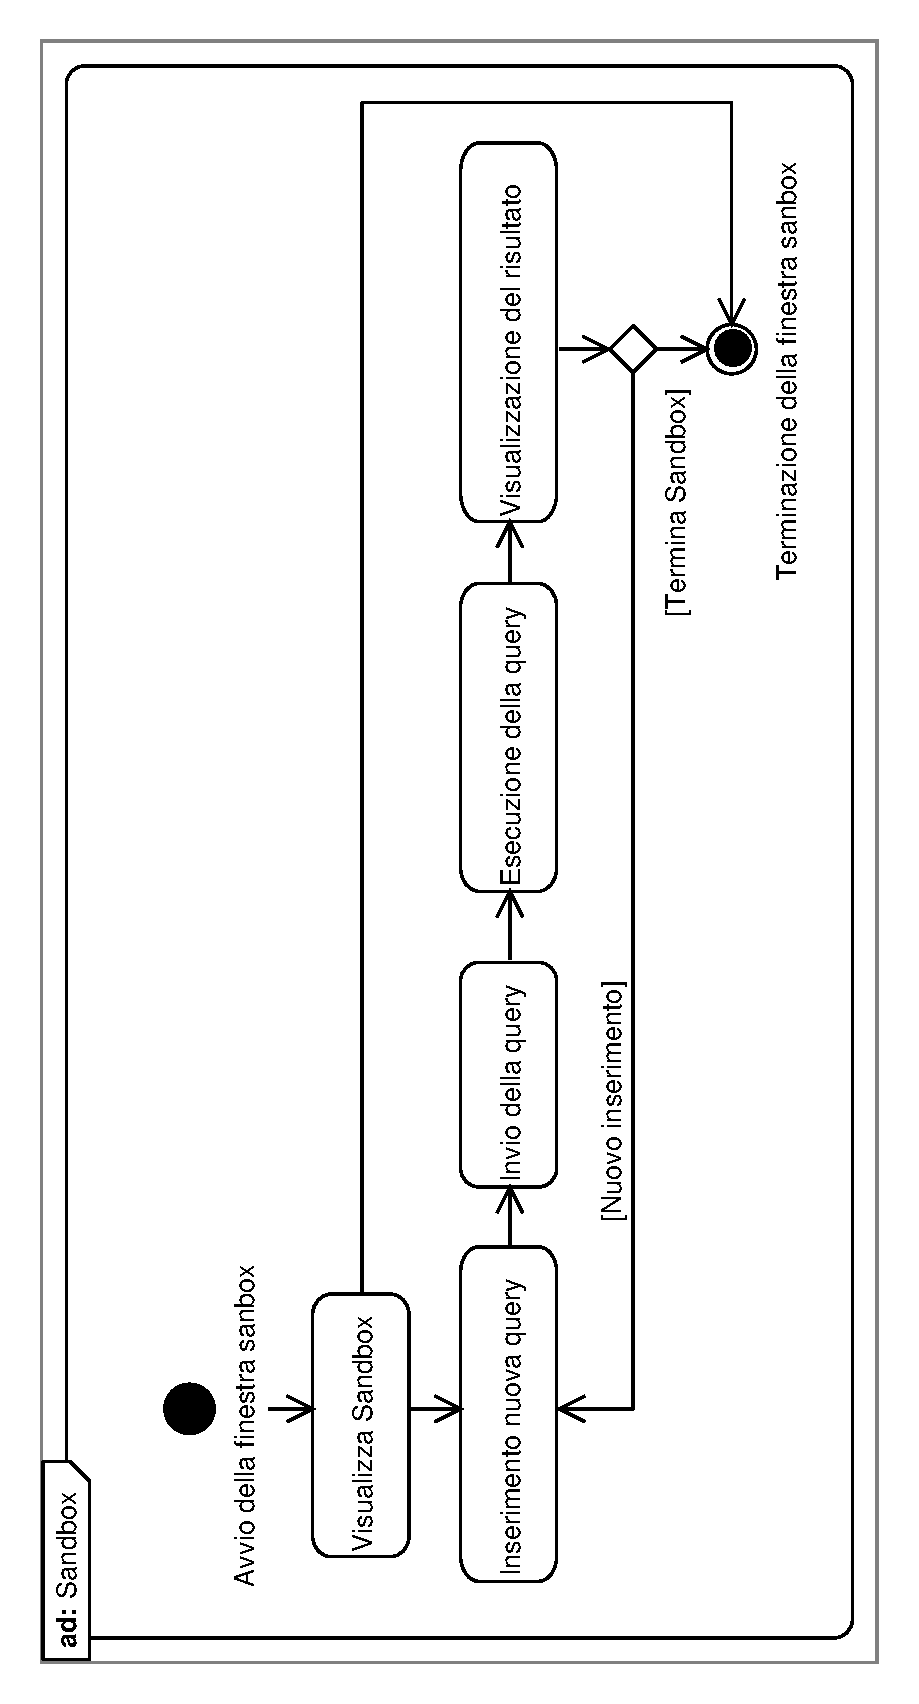
\includegraphics[width=0.5\textwidth, angle=-90]{activity-dia/Sandbox.eps}
\end{center}
La \textit{\underline{Sandbox}} \`e una finestra il cui scopo \`e permettere ad un utente di eseguire dei test sul repository. Viene quindi fornito uno spazio in cui digitare una query. La query viene inviata al \underline{DBMS} ed eseguita. Vengono infine presentati a video i risultati della query evidenziando il tempo impiegato per ottenerli. L'utente pu\`o poi terminare la finestra \textit{\underline{Sandbox}} o inserire una nuova query.

\subsection{Cancellazione \br}
\begin{center}
 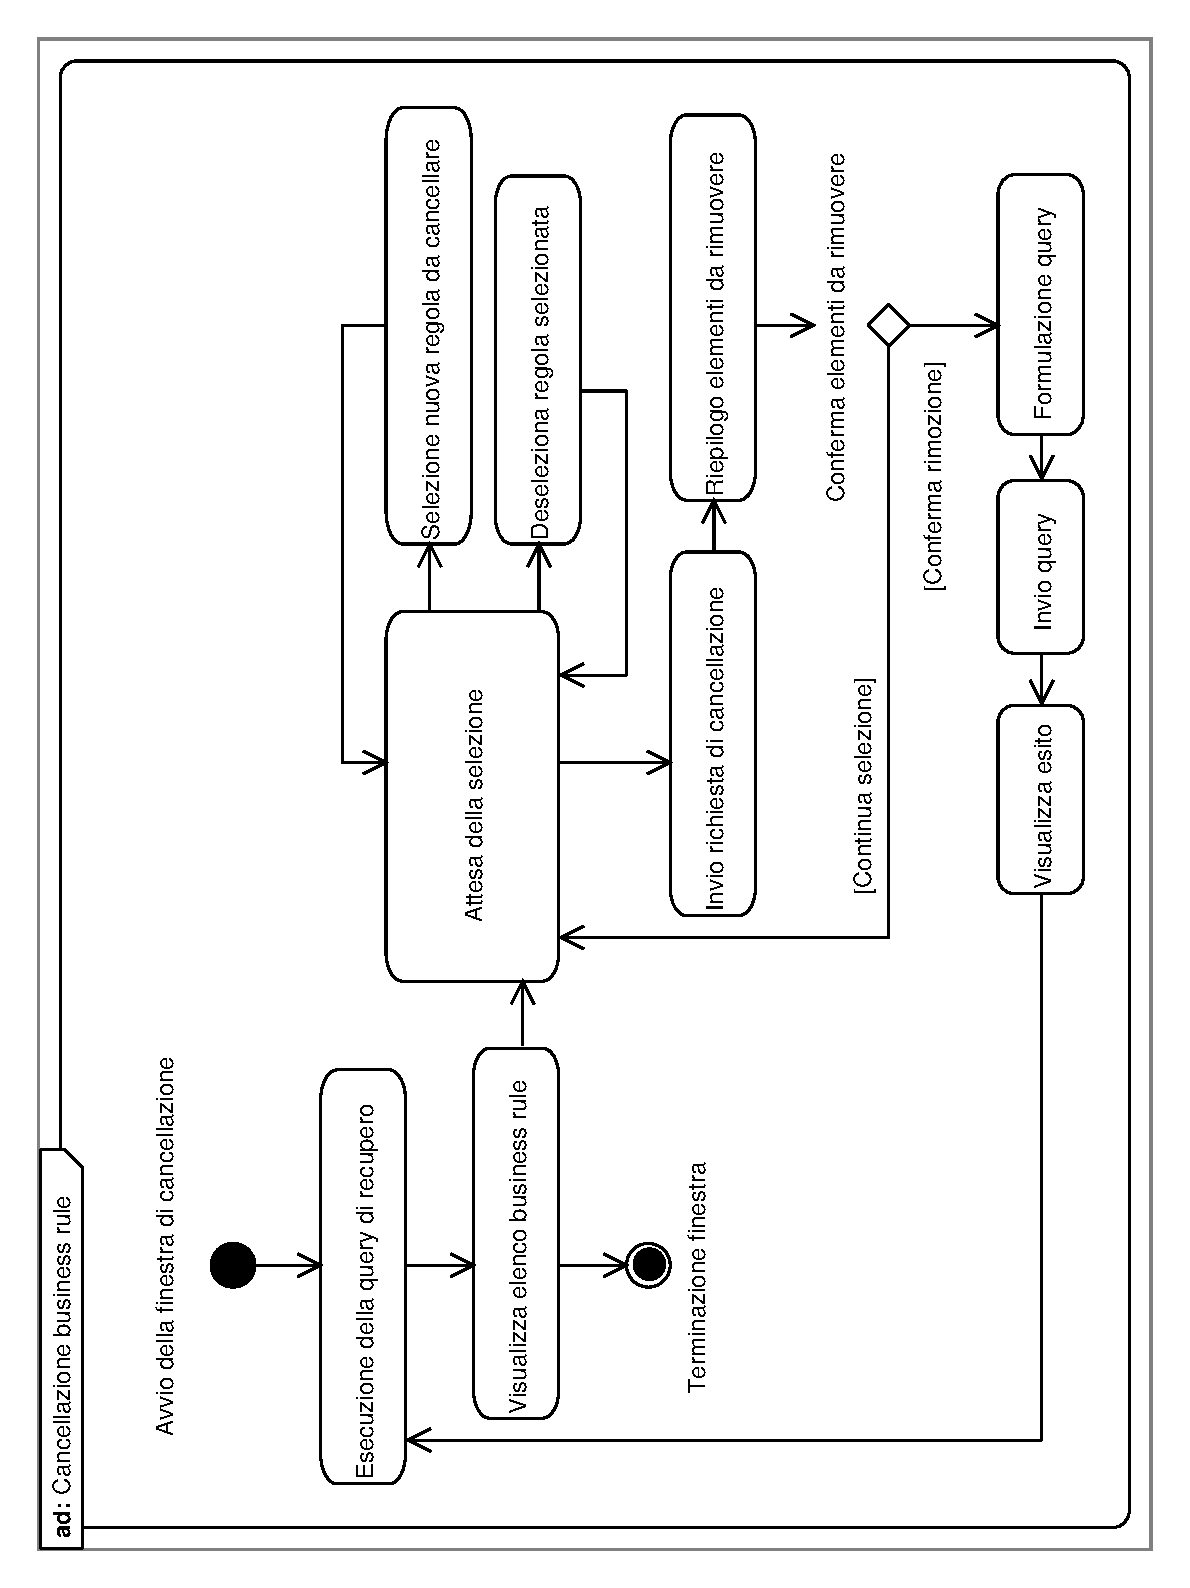
\includegraphics[width=0.7\textwidth, angle=-90]{activity-dia/CancellazioneBusinessRule.eps}
\end{center}
Viene inizialmente effettuata una query sul \underline{DBMS} atta a recuperare un elenco completo delle \br. Una volta recuperato l'elenco delle \br\ presenti nel \rp\ queste vengono visualizzate sinteticamente in forma tabellare, accompagnate da una \textit{checkbox}. Si attende quindi la selezione/deselezione dell'utente. L'utente notifica al sistema (mediante un bottone) l'intenzione di cancellare le \br\ selezionate.  Viene poi mostrato un riepilogo delle \br\ che verranno eliminate; se l'utente non conferma, il sistema torna ad attendere la selezione. Se, al contrario, la rimozione viene confermata si formula la query di rimozione, la quale viene infine eseguita. Al termine della rimozione viene effettuata nuovamente una query di recupero per visualizzare le \br\ rimaste nel \rp.

\section{Diagrammi di collaborazione}
Viene presentato di seguito un diagramma di collaborazione riguardante le relazioni tra le classi utilizzate nella cancellazione di una \br\ dal \rp.

\subsection{Cancellazione \br}
\begin{center}
 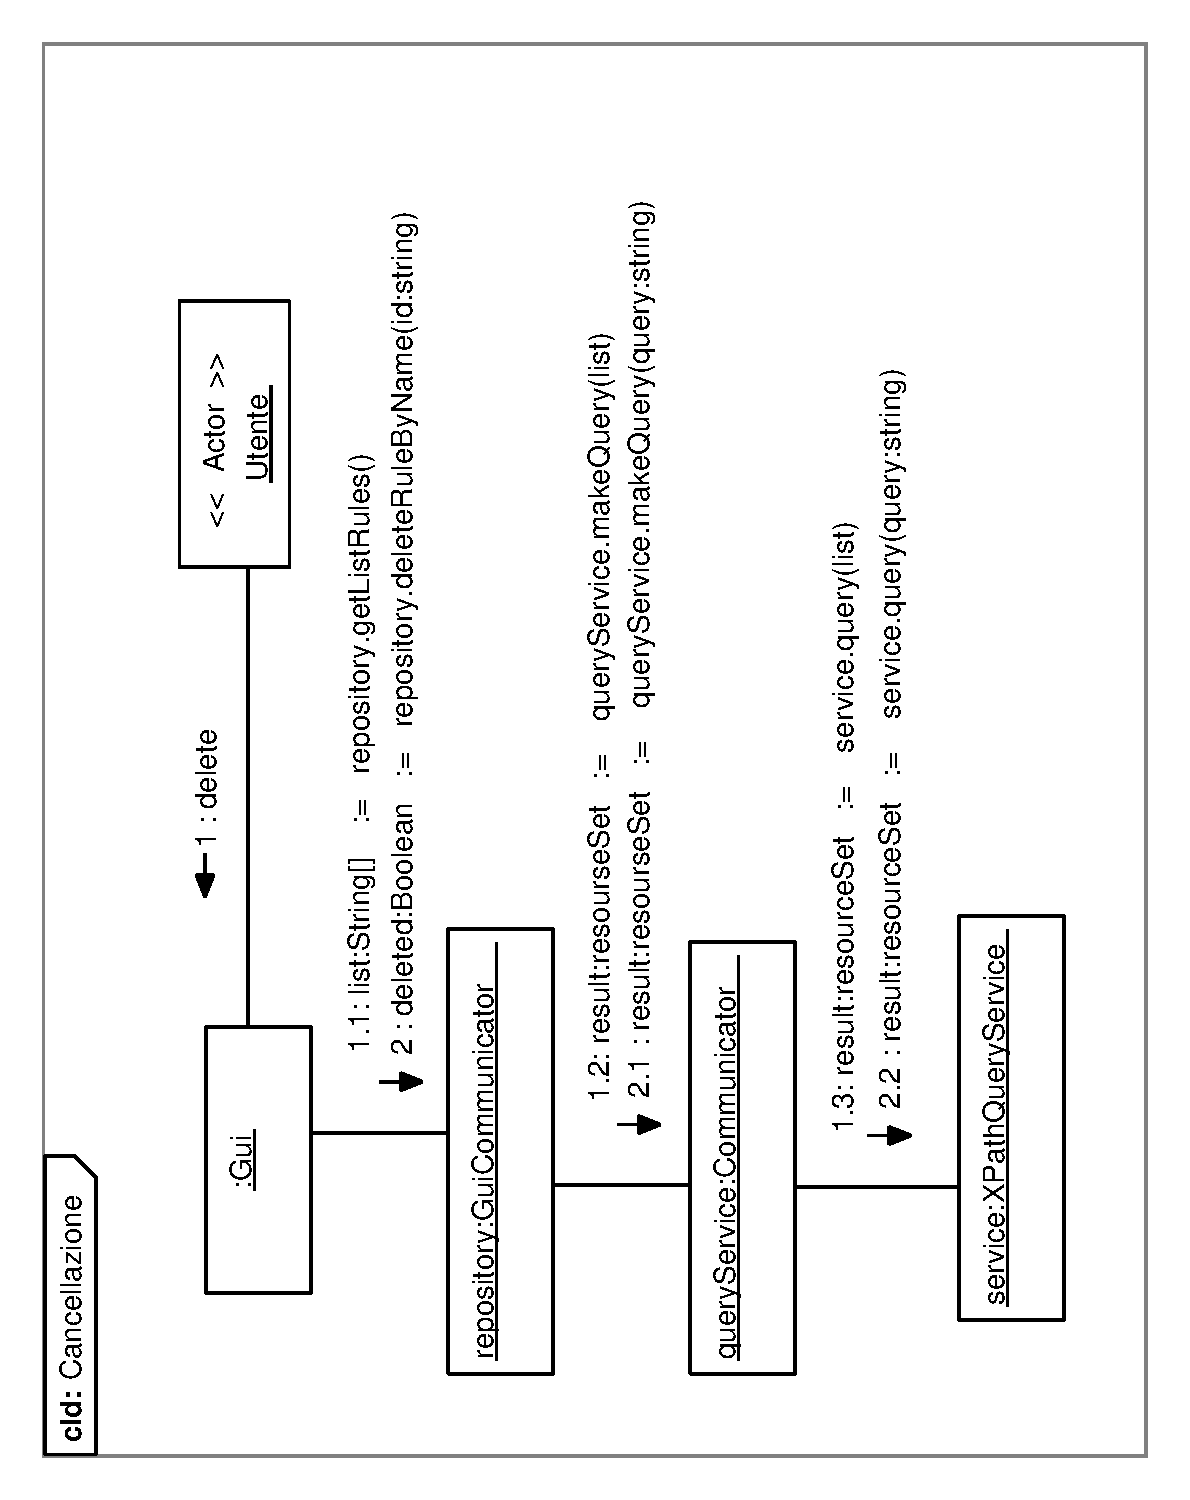
\includegraphics[width=0.8\textwidth, angle=-90]{collaboration-dia/Cancellazione.eps}
\end{center}
L'utente chiede di cancellare una \br\ alla GUI. Questa richiesta provoca innanzitutto l'invocazione di \textit{getListRules()} (1.1) sul campo dati \textit{\rp\ } della GUI. L'oggetto \rp\ che appartiene alla classe \textit{GuiCommunicator} invoca \textit{makeQuery(list)} (1.2) per recuperare la lista di \br\ dal \rp. Successivamente viene invocata \textit{query()} (1.3) sull'oggetto \textit{service} della classe \textit{XPathQuery} che si occupa di eseguire la query. Il risultato \`e riportato alla GUI mediante l'oggetto \textit{result} della classe \textit{ResourseSet} che contiene appunto il risultato della query eseguita. Una volta effettuta la selezione delle \br\ da rimuovere viene invocato il metodo \textit{deleteRuleByName(id)} (2). Vengono quindi invocati gli stessi metodi (2.1,2.2) utilizzati precedentemente, ma questa volta la query eseguita ritorner\`a un \textit{result} vuoto perch\`e \`e una query di cancellazione e quindi \textit{deleteRuleByName(id)} si limiter\`a a tornare un \textit{Boolean} indicante l'esito positivo o negativo della cancellazione.

\section{Diagrammi di sequenza}
Viene di seguito illustrato un diagramma di sequenza che chiarisce la sequenza di chiamate e invocazioni fatte dall'interprete nella richiesta di \br\ al sistema \textit{\underline{BR-jsys}}. Non riuscendo a definire operazioni interne diverse dalla ricorsione in \textit{Poseidon}, le operazioni interne \textit{costruzione query} e \textit{conversione} sono state realizzate con delle frecce vuote indicanti un messaggio asincrono, piuttosto che delle frecce piene. Tali messaggi sono da intendersi tuttavia come messaggi sincroni.
\subsection{Interpretazione}
\begin{center}
 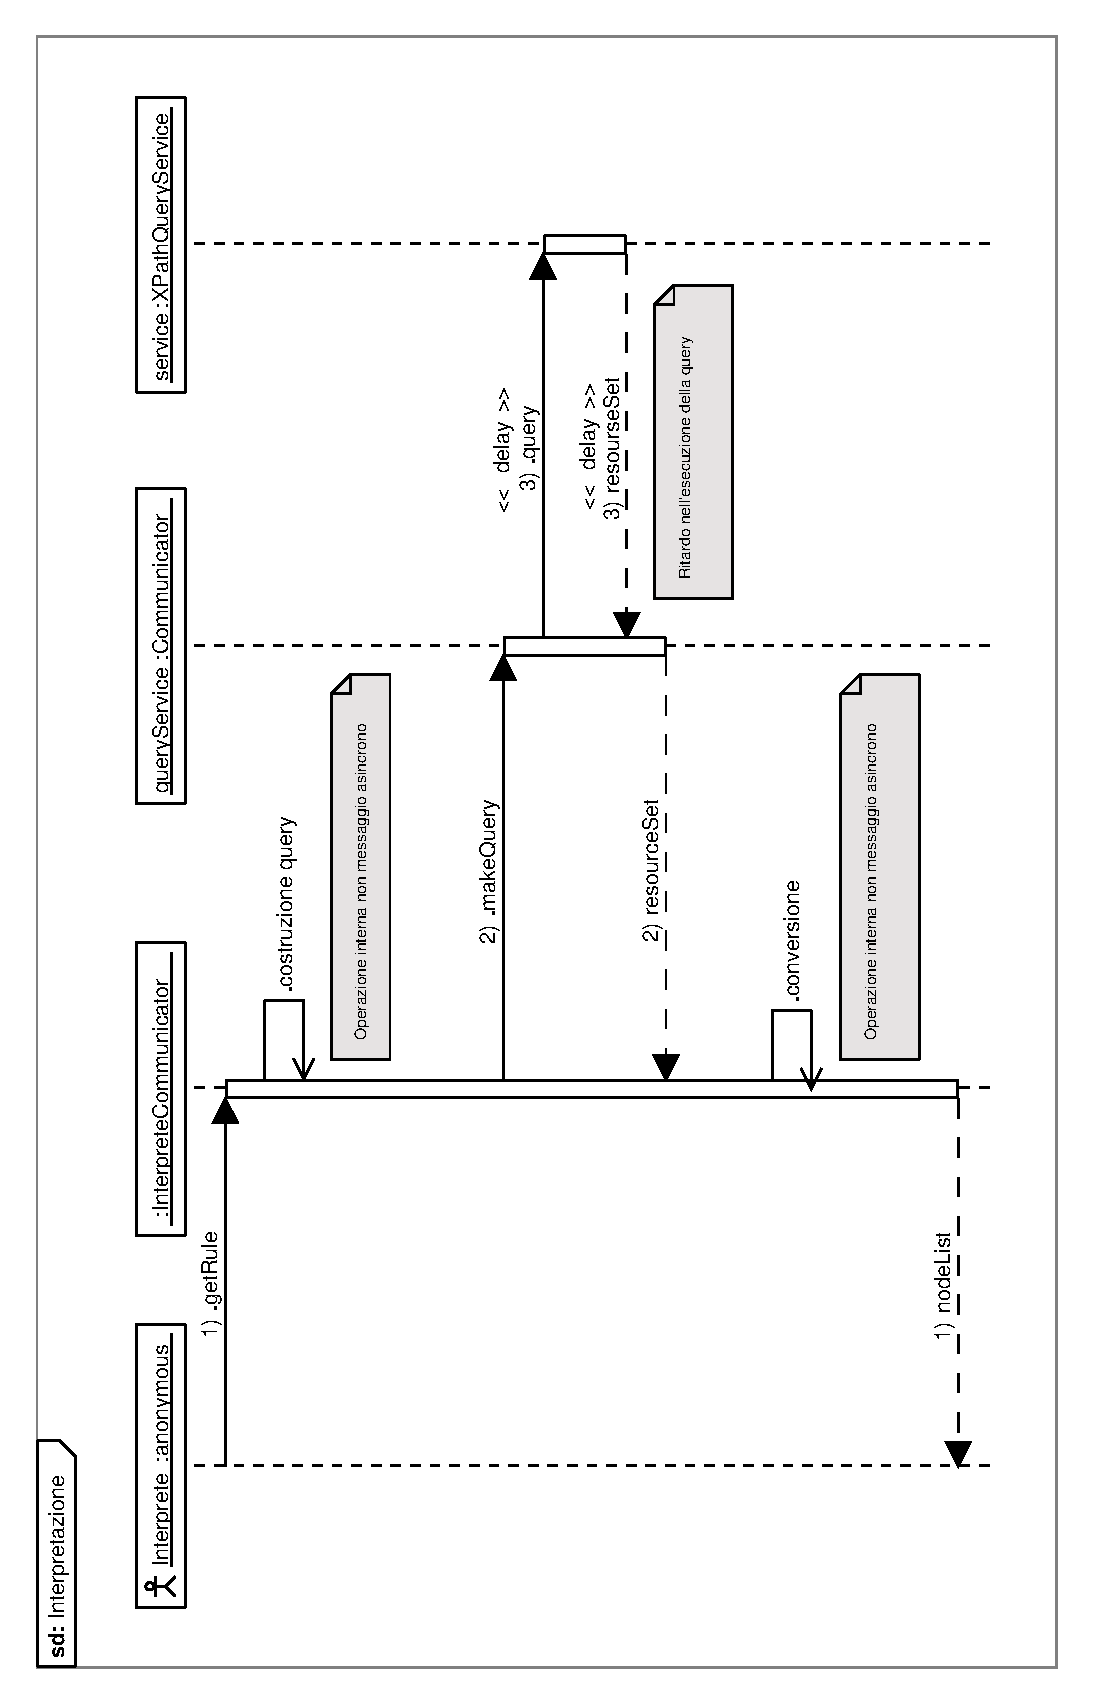
\includegraphics[width=0.6\textwidth, angle=-90]{sequence-dia/Interpretazione.eps}
\end{center}
L'interprete chiama \textit{getRule()} su un suo campo dati interno appartenente alla classe \textit{InterpreteCommunicator}. Il metodo getRule() \`e invocato con un parametro di tipo \textit{String} contenente il nome del \bo\ associato. Viene poi costruita la query lanciata mediante il metodo \textit{makeQuery} dell'oggetto \textit{queryService}. La query \`e poi eseguita dal metodo \textit{query} dell'oggetto \textit{service}. Viene quindi ritornato un \textit{resourceSet} che sar\`a convertito in un \textit{nodeList} e ritornato all'interprete. Il messaggio 3) \`e un messaggio con ritardo, ma non siamo riusciti a rappresentarlo con \textit{Poseidon}.

\section{Diagrammi di stato}

\subsection{Server DBMS}
\begin{center}
 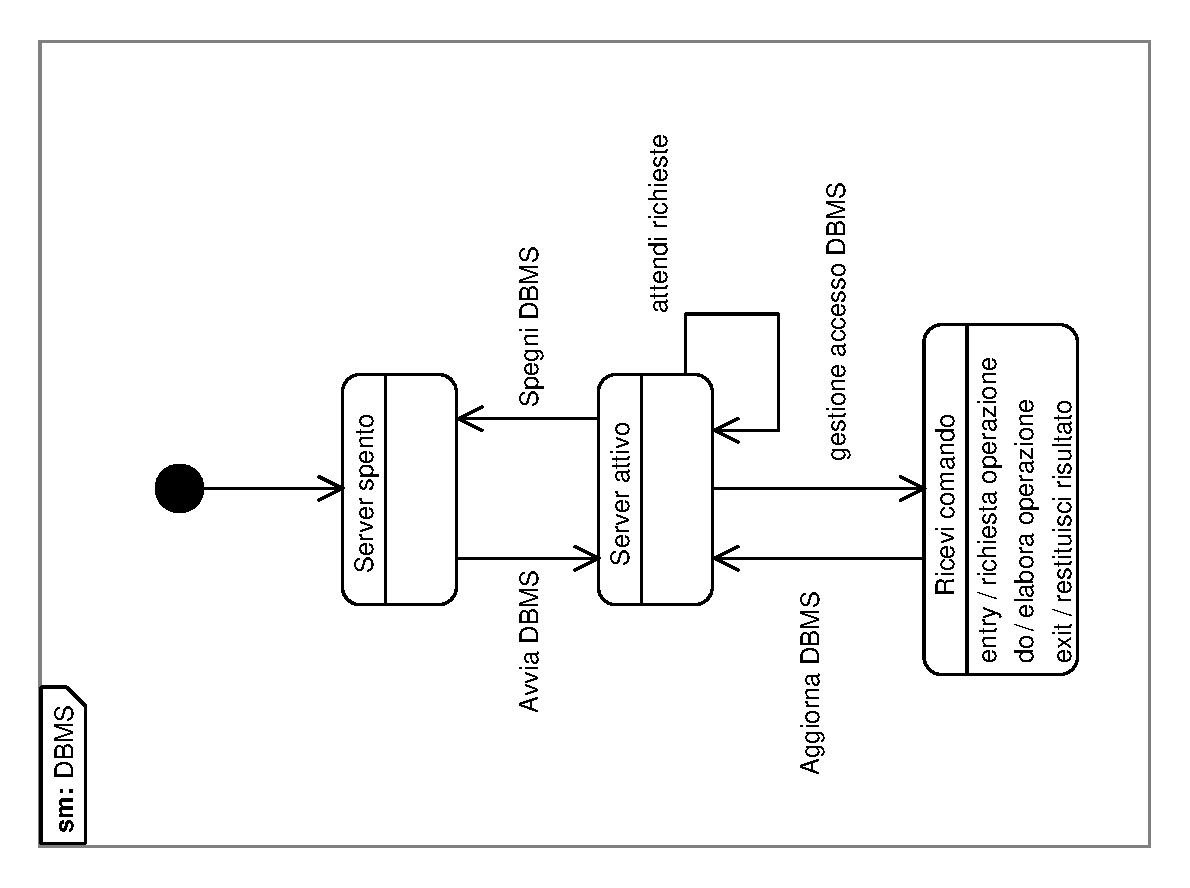
\includegraphics[width=0.9\textwidth, angle=-90]{state-dia/DBMS.eps}
\end{center}
Il server \underline{DBMS}, con il quale interagisce il prodotto ``\underline{BR-jsys}'', viene avviato. Una volta completata la procedura di avvio, entra in uno stato di attesa di richieste da parte del nostro prodotto. Ricevuta una richiesta di operazione(per esempio, una richiesta di connessione, di creazione del \rp\ o di accesso allo stesso), dovr\`a valutarla, eseguirla e ritornare i relativi risultati. Il server successivamente torna in uno stato di attesa finch\`e, eventualmente, viene spento.

\chapter{Stime di fattibilit\`a e di bisogno di risorse}
Dopo aver analizzato il problema attraverso schemi progettuali sono state individuate le risorse necessarie per la realizzazione del prodotto. Con l'utilizzo di software open source siamo riusciti a contenere i costi e contemporaneamente a rendere disponibili tutte le risorse.
Tutte le risorse necessarie ai nostri componenti per affrontare le varie problematiche di comunicazione, lo sviluppo del codice, la gestione degli archivi, la verifica dei documenti e del sistema, sono state descritte nel documento ``\PdQ''.
Nella fase di specifica tecnica e successivamente di progettazione verranno utilizzati diagrammi \underline{UML} realizzati con \textit{Poseidon for \underline{UML} Professional edition 6.0.2} (nella versione trial), in quanto pi\`u completo e usabile rispetto ad altri software simili, come ad esempio ArgoUML. Solo i diagrammi use case sono stati realizzati con Dia in quanto progettati prima di affidarsi a Poseidon.
Il progetto sar\`a realizzato mediante il linguaggio java come da requisito implicito del capitolato. Useremo la versione 6 essendo quella di pi\`u recente sviluppo.
Per la produzione della Gui e delle classi java abbiamo utilizzato Eclipse versione 3.3.1.1, un IDE in grado di fornire numerose funzionalit\`a per lo sviluppo del software.
Per la parte riguardante la grammatica, dopo varie ricerche e confronti, ci siamo affidati invece ad \underline{Antlr} 3.0.1 come generatore di parser e AntlrWorks 1.1.5 come ambiente grafico di sviluppo in quanto offrivano la maggior chiarezza e risposta alle nostre aspettative.
Tutta la documentazione sar\`a redatta utilizzando Kile 2.0 un user-friendly Tex/Latex editor completo e chiaro nelle sue funzionalit\`a.
Lo sviluppo avr\`a luogo singolarmente o in piccoli gruppi a seconda della natura della problematica da affrontare.
Il documento/codice avr\`a ad ogni modo un unico proprietario incaricato di renderlo pubblico tramite server SVN.
Utilizzando queste risorse e visti i tempi di consegna del prodotto, la ditta HappyCode ritiene quindi soddisfacibili le richieste del proponente.
Per tempistiche pi\`u dettagliate si rimanda al ``\PdP''.

\chapter{Appendice}
\section{Tracciamento della relazione componenti - ~requisiti}
\begin{center}
\large{
\begin{tabular}{l}
\begin{tabular}{||p{2.6cm}||p{4.6cm}||p{2.8cm}||} \hline
\textbf{Componente} & \textbf{Componente Specifico} & \textbf{Requisiti Associati} \\ \hline

GUI & & F4, F5, F7, F8\\ \hline
 &  & \\ \hline

Validatore & Validator & F2, F3, F4, F5, F8, NPR1, NQ1\\ \hline
 & BusinessRuleLexer & F2, F4, NQ1 \\ \hline
 & BusinessRuleParser & F2, F4, F10, NQ1 \\ \hline
 & TypeCollisionException & F2, F4, F10, NQ1\\ \hline
 & XMLParser & NPo1\\ \hline
 & businessobjects & F2, F10, F11\\ \hline
 &  & \\ \hline

BusinessRule & & F2, F10, F11, NU1, NU2, NU3, NQ1\\ \hline
 &  & \\ \hline

Comunicatore & Communicator & F3, F5, F6, NPr1\\ \hline
 & GUICommunicator & F5, F7, F8\\ \hline
 & InterpreterCommunicator & F5, F6\\ \hline
 & ValidatorCommunicator & F3\\ \hline

\end{tabular} \\
\end{tabular}

}
\end{center}


\section{Tracciamento della relazione inversa: requisiti - componenti}

\begin{center}


\large{
\begin{tabular}{l}
\begin{tabular}{||p{3cm}||p{9cm}||} \hline
\textbf{Requisito} & {Componenti associati} \\ \hline
\textbf{F2} & Validator, BusinessRuleLexer, BusinessRuleParser, TypeCollisionException, businessobject, BusinessRule \\ \hline
\textbf{F3} & Validator, Communicator, ValidatorCommunicator \\ \hline
\textbf{F4} & GUI, Validator, BusinessRuleLexer, BusinessRuleParser, TypeCollisionException \\ \hline
\textbf{F5} & GUI, Validator, Communicator, GUICommunicator, InterpreterCommunicator, \\ \hline
\textbf{F6} & Communicator, InterpreterCommunicator \\ \hline
\textbf{F7} & GUI, GUICommunicator \\ \hline
\textbf{F8} & GUI, Validator, GUICommunicator \\ \hline
\textbf{F10} & BusinessRuleParser, TypeCollisionException, businessobject, \underline{Business Rule} \\ \hline
\textbf{F11} & businessobject, \underline{Business Rule} \\ \hline
\textbf{NU1} & BusinessRule \\ \hline
\textbf{NU2} & BusinessRule \\ \hline
\textbf{NU3} & BusinessRule \\ \hline
\textbf{NPo1} &  XMLParser \\ \hline
\textbf{NPr1} & Validator, Communicator \\ \hline
\textbf{NQ1} & Validator, BusinessRuleLexer, BusinessRuleParser, TypeCollisionException, BusinessRule \\ \hline
\end{tabular} \\
\end{tabular}
}
\end{center}

\end{document}
